% Options for packages loaded elsewhere
\PassOptionsToPackage{unicode}{hyperref}
\PassOptionsToPackage{hyphens}{url}
\PassOptionsToPackage{dvipsnames,svgnames,x11names}{xcolor}
%
\documentclass[
  letterpaper,
  DIV=11,
  numbers=noendperiod]{scrartcl}

\usepackage{amsmath,amssymb}
\usepackage{iftex}
\ifPDFTeX
  \usepackage[T1]{fontenc}
  \usepackage[utf8]{inputenc}
  \usepackage{textcomp} % provide euro and other symbols
\else % if luatex or xetex
  \usepackage{unicode-math}
  \defaultfontfeatures{Scale=MatchLowercase}
  \defaultfontfeatures[\rmfamily]{Ligatures=TeX,Scale=1}
\fi
\usepackage{lmodern}
\ifPDFTeX\else  
    % xetex/luatex font selection
\fi
% Use upquote if available, for straight quotes in verbatim environments
\IfFileExists{upquote.sty}{\usepackage{upquote}}{}
\IfFileExists{microtype.sty}{% use microtype if available
  \usepackage[]{microtype}
  \UseMicrotypeSet[protrusion]{basicmath} % disable protrusion for tt fonts
}{}
\makeatletter
\@ifundefined{KOMAClassName}{% if non-KOMA class
  \IfFileExists{parskip.sty}{%
    \usepackage{parskip}
  }{% else
    \setlength{\parindent}{0pt}
    \setlength{\parskip}{6pt plus 2pt minus 1pt}}
}{% if KOMA class
  \KOMAoptions{parskip=half}}
\makeatother
\usepackage{xcolor}
\setlength{\emergencystretch}{3em} % prevent overfull lines
\setcounter{secnumdepth}{-\maxdimen} % remove section numbering
% Make \paragraph and \subparagraph free-standing
\makeatletter
\ifx\paragraph\undefined\else
  \let\oldparagraph\paragraph
  \renewcommand{\paragraph}{
    \@ifstar
      \xxxParagraphStar
      \xxxParagraphNoStar
  }
  \newcommand{\xxxParagraphStar}[1]{\oldparagraph*{#1}\mbox{}}
  \newcommand{\xxxParagraphNoStar}[1]{\oldparagraph{#1}\mbox{}}
\fi
\ifx\subparagraph\undefined\else
  \let\oldsubparagraph\subparagraph
  \renewcommand{\subparagraph}{
    \@ifstar
      \xxxSubParagraphStar
      \xxxSubParagraphNoStar
  }
  \newcommand{\xxxSubParagraphStar}[1]{\oldsubparagraph*{#1}\mbox{}}
  \newcommand{\xxxSubParagraphNoStar}[1]{\oldsubparagraph{#1}\mbox{}}
\fi
\makeatother

\usepackage{color}
\usepackage{fancyvrb}
\newcommand{\VerbBar}{|}
\newcommand{\VERB}{\Verb[commandchars=\\\{\}]}
\DefineVerbatimEnvironment{Highlighting}{Verbatim}{commandchars=\\\{\}}
% Add ',fontsize=\small' for more characters per line
\usepackage{framed}
\definecolor{shadecolor}{RGB}{241,243,245}
\newenvironment{Shaded}{\begin{snugshade}}{\end{snugshade}}
\newcommand{\AlertTok}[1]{\textcolor[rgb]{0.68,0.00,0.00}{#1}}
\newcommand{\AnnotationTok}[1]{\textcolor[rgb]{0.37,0.37,0.37}{#1}}
\newcommand{\AttributeTok}[1]{\textcolor[rgb]{0.40,0.45,0.13}{#1}}
\newcommand{\BaseNTok}[1]{\textcolor[rgb]{0.68,0.00,0.00}{#1}}
\newcommand{\BuiltInTok}[1]{\textcolor[rgb]{0.00,0.23,0.31}{#1}}
\newcommand{\CharTok}[1]{\textcolor[rgb]{0.13,0.47,0.30}{#1}}
\newcommand{\CommentTok}[1]{\textcolor[rgb]{0.37,0.37,0.37}{#1}}
\newcommand{\CommentVarTok}[1]{\textcolor[rgb]{0.37,0.37,0.37}{\textit{#1}}}
\newcommand{\ConstantTok}[1]{\textcolor[rgb]{0.56,0.35,0.01}{#1}}
\newcommand{\ControlFlowTok}[1]{\textcolor[rgb]{0.00,0.23,0.31}{\textbf{#1}}}
\newcommand{\DataTypeTok}[1]{\textcolor[rgb]{0.68,0.00,0.00}{#1}}
\newcommand{\DecValTok}[1]{\textcolor[rgb]{0.68,0.00,0.00}{#1}}
\newcommand{\DocumentationTok}[1]{\textcolor[rgb]{0.37,0.37,0.37}{\textit{#1}}}
\newcommand{\ErrorTok}[1]{\textcolor[rgb]{0.68,0.00,0.00}{#1}}
\newcommand{\ExtensionTok}[1]{\textcolor[rgb]{0.00,0.23,0.31}{#1}}
\newcommand{\FloatTok}[1]{\textcolor[rgb]{0.68,0.00,0.00}{#1}}
\newcommand{\FunctionTok}[1]{\textcolor[rgb]{0.28,0.35,0.67}{#1}}
\newcommand{\ImportTok}[1]{\textcolor[rgb]{0.00,0.46,0.62}{#1}}
\newcommand{\InformationTok}[1]{\textcolor[rgb]{0.37,0.37,0.37}{#1}}
\newcommand{\KeywordTok}[1]{\textcolor[rgb]{0.00,0.23,0.31}{\textbf{#1}}}
\newcommand{\NormalTok}[1]{\textcolor[rgb]{0.00,0.23,0.31}{#1}}
\newcommand{\OperatorTok}[1]{\textcolor[rgb]{0.37,0.37,0.37}{#1}}
\newcommand{\OtherTok}[1]{\textcolor[rgb]{0.00,0.23,0.31}{#1}}
\newcommand{\PreprocessorTok}[1]{\textcolor[rgb]{0.68,0.00,0.00}{#1}}
\newcommand{\RegionMarkerTok}[1]{\textcolor[rgb]{0.00,0.23,0.31}{#1}}
\newcommand{\SpecialCharTok}[1]{\textcolor[rgb]{0.37,0.37,0.37}{#1}}
\newcommand{\SpecialStringTok}[1]{\textcolor[rgb]{0.13,0.47,0.30}{#1}}
\newcommand{\StringTok}[1]{\textcolor[rgb]{0.13,0.47,0.30}{#1}}
\newcommand{\VariableTok}[1]{\textcolor[rgb]{0.07,0.07,0.07}{#1}}
\newcommand{\VerbatimStringTok}[1]{\textcolor[rgb]{0.13,0.47,0.30}{#1}}
\newcommand{\WarningTok}[1]{\textcolor[rgb]{0.37,0.37,0.37}{\textit{#1}}}

\providecommand{\tightlist}{%
  \setlength{\itemsep}{0pt}\setlength{\parskip}{0pt}}\usepackage{longtable,booktabs,array}
\usepackage{calc} % for calculating minipage widths
% Correct order of tables after \paragraph or \subparagraph
\usepackage{etoolbox}
\makeatletter
\patchcmd\longtable{\par}{\if@noskipsec\mbox{}\fi\par}{}{}
\makeatother
% Allow footnotes in longtable head/foot
\IfFileExists{footnotehyper.sty}{\usepackage{footnotehyper}}{\usepackage{footnote}}
\makesavenoteenv{longtable}
\usepackage{graphicx}
\makeatletter
\newsavebox\pandoc@box
\newcommand*\pandocbounded[1]{% scales image to fit in text height/width
  \sbox\pandoc@box{#1}%
  \Gscale@div\@tempa{\textheight}{\dimexpr\ht\pandoc@box+\dp\pandoc@box\relax}%
  \Gscale@div\@tempb{\linewidth}{\wd\pandoc@box}%
  \ifdim\@tempb\p@<\@tempa\p@\let\@tempa\@tempb\fi% select the smaller of both
  \ifdim\@tempa\p@<\p@\scalebox{\@tempa}{\usebox\pandoc@box}%
  \else\usebox{\pandoc@box}%
  \fi%
}
% Set default figure placement to htbp
\def\fps@figure{htbp}
\makeatother

\usepackage{float}
\usepackage{tabularray}
\usepackage[normalem]{ulem}
\usepackage{graphicx}
\UseTblrLibrary{booktabs}
\UseTblrLibrary{rotating}
\UseTblrLibrary{siunitx}
\NewTableCommand{\tinytableDefineColor}[3]{\definecolor{#1}{#2}{#3}}
\newcommand{\tinytableTabularrayUnderline}[1]{\underline{#1}}
\newcommand{\tinytableTabularrayStrikeout}[1]{\sout{#1}}
\usepackage{fvextra}
\DefineVerbatimEnvironment{Highlighting}{Verbatim}{breaklines,commandchars=\\\{\}}
\DefineVerbatimEnvironment{OutputCode}{Verbatim}{breaklines,commandchars=\\\{\}}
\KOMAoption{captions}{tableheading}
\makeatletter
\@ifpackageloaded{caption}{}{\usepackage{caption}}
\AtBeginDocument{%
\ifdefined\contentsname
  \renewcommand*\contentsname{Table of contents}
\else
  \newcommand\contentsname{Table of contents}
\fi
\ifdefined\listfigurename
  \renewcommand*\listfigurename{List of Figures}
\else
  \newcommand\listfigurename{List of Figures}
\fi
\ifdefined\listtablename
  \renewcommand*\listtablename{List of Tables}
\else
  \newcommand\listtablename{List of Tables}
\fi
\ifdefined\figurename
  \renewcommand*\figurename{Figure}
\else
  \newcommand\figurename{Figure}
\fi
\ifdefined\tablename
  \renewcommand*\tablename{Table}
\else
  \newcommand\tablename{Table}
\fi
}
\@ifpackageloaded{float}{}{\usepackage{float}}
\floatstyle{ruled}
\@ifundefined{c@chapter}{\newfloat{codelisting}{h}{lop}}{\newfloat{codelisting}{h}{lop}[chapter]}
\floatname{codelisting}{Listing}
\newcommand*\listoflistings{\listof{codelisting}{List of Listings}}
\makeatother
\makeatletter
\makeatother
\makeatletter
\@ifpackageloaded{caption}{}{\usepackage{caption}}
\@ifpackageloaded{subcaption}{}{\usepackage{subcaption}}
\makeatother

\usepackage{bookmark}

\IfFileExists{xurl.sty}{\usepackage{xurl}}{} % add URL line breaks if available
\urlstyle{same} % disable monospaced font for URLs
\hypersetup{
  pdftitle={Problem set 3},
  pdfauthor={Hyoungchul Kim},
  colorlinks=true,
  linkcolor={blue},
  filecolor={Maroon},
  citecolor={Blue},
  urlcolor={Blue},
  pdfcreator={LaTeX via pandoc}}


\title{Problem set 3}
\author{Hyoungchul Kim}
\date{2025-04-03}

\begin{document}
\maketitle


\section{Replications}\label{replications}

\subsection{Q1}\label{q1}

This paper examines the impact of unilateral divorce on various outcomes
such as family violence, reported suicide and spousal homicide. The
estimating equation they employ are DiD. They use TWFE model as follows

\[
\text{suicide}_{s,t} = \sum_k \beta_k \, \text{unilateral}_{s,t}^k + \text{state}_s + \text{year}_t + \text{control}_{s,t} + \varepsilon_{s,t}.
\]

To be exact, it is dynamic TWFE because we are estimating coefficients
for all periods after the treatment. The necessary assumption is
parallel trends and no anticiaption. That is, the evolution of the
outcome of interest should have been in same magnitude for both
treatment and control groups in absence of the treatment. While the
assumption seems bit plausible, the problem in this case would be the
fact that there can be negative weighting problem for the staggered DiD
TWFE model. For the negative weighting problem, we would have to do the
new DiD methods to alleviate it. Another possible concern with the
identification assumption would be that there can be some confounding
factor that is correlated with the treatment. It might be good to check
if there were any change in policy that might have happened when the
unilateral divorce policy change was happening.

\subsection{Q2}\label{q2}

Read in the data:

\begin{Shaded}
\begin{Highlighting}[]
\NormalTok{data }\OtherTok{\textless{}{-}}\NormalTok{ haven}\SpecialCharTok{::}\FunctionTok{read\_dta}\NormalTok{(}\StringTok{"data/divorce\_example.dta"}\NormalTok{)}
\end{Highlighting}
\end{Shaded}

Do some sum stat for suicide rates for men and women (\texttt{asmrs}).
We also do sum stat for policy indicator (\texttt{post}):

\begin{Shaded}
\begin{Highlighting}[]
\FunctionTok{library}\NormalTok{(data.table)}
\FunctionTok{library}\NormalTok{(tidyverse)}
\FunctionTok{library}\NormalTok{(modelsummary)}
\FunctionTok{setDT}\NormalTok{(data)}

\NormalTok{data }\OtherTok{\textless{}{-}}\NormalTok{ data }\SpecialCharTok{\%\textgreater{}\%}
  \FunctionTok{mutate}\NormalTok{(}
    \AttributeTok{post =} \FunctionTok{if\_else}\NormalTok{(year }\SpecialCharTok{\textgreater{}=}\NormalTok{ nfd, }\DecValTok{1}\NormalTok{, }\DecValTok{0}\NormalTok{),}
    \AttributeTok{post =} \FunctionTok{if\_else}\NormalTok{(nfd }\SpecialCharTok{==} \StringTok{"PRE"}\NormalTok{, }\DecValTok{1}\NormalTok{, post)}
\NormalTok{  )}

\CommentTok{\# 1. Summary of asmrs by sex}
\NormalTok{asmrs\_tbl }\OtherTok{\textless{}{-}} \FunctionTok{datasummary\_df}\NormalTok{(}
\NormalTok{  data }\SpecialCharTok{\%\textgreater{}\%}
    \FunctionTok{mutate}\NormalTok{(}\AttributeTok{sex=}\FunctionTok{ifelse}\NormalTok{(sex}\SpecialCharTok{==}\DecValTok{1}\NormalTok{, }\StringTok{"male"}\NormalTok{, }\StringTok{"female"}\NormalTok{)) }\SpecialCharTok{\%\textgreater{}\%} 
    \FunctionTok{group\_by}\NormalTok{(sex) }\SpecialCharTok{\%\textgreater{}\%}
    \FunctionTok{summarise}\NormalTok{(}
      \AttributeTok{Mean =} \FunctionTok{mean}\NormalTok{(asmrs, }\AttributeTok{na.rm =} \ConstantTok{TRUE}\NormalTok{),}
      \AttributeTok{SD =} \FunctionTok{sd}\NormalTok{(asmrs, }\AttributeTok{na.rm =} \ConstantTok{TRUE}\NormalTok{),}
      \AttributeTok{N =} \FunctionTok{n}\NormalTok{()}
\NormalTok{    ) }\SpecialCharTok{\%\textgreater{}\%}
    \FunctionTok{mutate}\NormalTok{(}\AttributeTok{variable =} \StringTok{"asmrs"}\NormalTok{) }\SpecialCharTok{\%\textgreater{}\%}
    \FunctionTok{select}\NormalTok{(variable, }\FunctionTok{everything}\NormalTok{()),}
  \AttributeTok{output =} \StringTok{"data.frame"}
\NormalTok{)}

\CommentTok{\# 2. Summary of post (no grouping)}
\NormalTok{post\_tbl }\OtherTok{\textless{}{-}} \FunctionTok{datasummary\_df}\NormalTok{(}
\NormalTok{  data }\SpecialCharTok{\%\textgreater{}\%}
    \FunctionTok{mutate}\NormalTok{(}\AttributeTok{sex=}\FunctionTok{ifelse}\NormalTok{(sex}\SpecialCharTok{==}\DecValTok{1}\NormalTok{, }\StringTok{"male"}\NormalTok{, }\StringTok{"female"}\NormalTok{)) }\SpecialCharTok{\%\textgreater{}\%} 
    \FunctionTok{summarise}\NormalTok{(}
      \AttributeTok{Mean =} \FunctionTok{mean}\NormalTok{(post, }\AttributeTok{na.rm =} \ConstantTok{TRUE}\NormalTok{),}
      \AttributeTok{SD =} \FunctionTok{sd}\NormalTok{(post, }\AttributeTok{na.rm =} \ConstantTok{TRUE}\NormalTok{),}
      \AttributeTok{N =} \FunctionTok{n}\NormalTok{()}
\NormalTok{    ) }\SpecialCharTok{\%\textgreater{}\%}
    \FunctionTok{mutate}\NormalTok{(}\AttributeTok{variable =} \StringTok{"post"}\NormalTok{) }\SpecialCharTok{\%\textgreater{}\%}
    \FunctionTok{select}\NormalTok{(variable, }\FunctionTok{everything}\NormalTok{()),}
  \AttributeTok{output =} \StringTok{"data.frame"}
\NormalTok{)}

\CommentTok{\# 3. Combine both tables}
\NormalTok{combined\_tbl }\OtherTok{\textless{}{-}} \FunctionTok{bind\_rows}\NormalTok{(asmrs\_tbl, post\_tbl)}

\CommentTok{\# 4. Show as a table}
\FunctionTok{datasummary\_df}\NormalTok{(combined\_tbl, }\AttributeTok{output =} \StringTok{"markdown"}\NormalTok{)}
\end{Highlighting}
\end{Shaded}

\begin{table}
\centering
\begin{tblr}[         %% tabularray outer open
]                     %% tabularray outer close
{                     %% tabularray inner open
colspec={Q[]Q[]Q[]Q[]Q[]},
column{1,2,3,4,5}={}{halign=l,},
}                     %% tabularray inner close
\toprule
variable & sex & Mean & SD & N \\ \midrule %% TinyTableHeader
asmrs & female & 5.06  & 2.88 & 2301.00 \\
asmrs & male   & 18.48 & 8.33 & 2301.00 \\
post  & NA     & 0.53  & 0.50 & 4602.00 \\
\bottomrule
\end{tblr}
\end{table}

\subsection{Q3}\label{q3}

Now we will just run a simple TWFE model.

\begin{Shaded}
\begin{Highlighting}[]
\FunctionTok{library}\NormalTok{(fixest) }
\FunctionTok{library}\NormalTok{(texreg)}

\NormalTok{data }\OtherTok{\textless{}{-}}\NormalTok{ data }\SpecialCharTok{\%\textgreater{}\%} \FunctionTok{filter}\NormalTok{(year}\SpecialCharTok{\textgreater{}=}\DecValTok{1964} \SpecialCharTok{\&}\NormalTok{ year}\SpecialCharTok{\textless{}=} \DecValTok{1996}\NormalTok{)}

\NormalTok{data }\OtherTok{\textless{}{-}}\NormalTok{ data }\SpecialCharTok{\%\textgreater{}\%} \FunctionTok{mutate}\NormalTok{(}\AttributeTok{year\_post =}\NormalTok{ year }\SpecialCharTok{{-}} \StringTok{\textasciigrave{}}\AttributeTok{\_nfd}\StringTok{\textasciigrave{}}\NormalTok{)}
\NormalTok{data }\OtherTok{\textless{}{-}}\NormalTok{ data }\SpecialCharTok{\%\textgreater{}\%} \FunctionTok{mutate}\NormalTok{(}\AttributeTok{year\_post =} \FunctionTok{ifelse}\NormalTok{(year\_post }\SpecialCharTok{\textgreater{}=}\DecValTok{19} \SpecialCharTok{|}\NormalTok{ nfd }\SpecialCharTok{==} \StringTok{"PRE"}\NormalTok{, }\DecValTok{19}\NormalTok{, year\_post))}
\NormalTok{data }\OtherTok{\textless{}{-}}\NormalTok{ data }\SpecialCharTok{\%\textgreater{}\%} \FunctionTok{mutate}\NormalTok{(}\AttributeTok{year\_post =} \FunctionTok{ifelse}\NormalTok{(year\_post }\SpecialCharTok{\textless{}} \DecValTok{0} \SpecialCharTok{|}\NormalTok{ nfd }\SpecialCharTok{==} \StringTok{"NRS"}\NormalTok{, }\DecValTok{100}\NormalTok{, year\_post))}

\NormalTok{data }\OtherTok{\textless{}{-}}\NormalTok{ data }\SpecialCharTok{\%\textgreater{}\%} 
  \FunctionTok{mutate}\NormalTok{(}
    \AttributeTok{cat\_post =} \FunctionTok{case\_when}\NormalTok{(}
\NormalTok{      year\_post }\SpecialCharTok{==} \DecValTok{0} \SpecialCharTok{\textasciitilde{}} \DecValTok{0}\NormalTok{,}
\NormalTok{      year\_post }\SpecialCharTok{==} \DecValTok{1} \SpecialCharTok{|}\NormalTok{ year\_post }\SpecialCharTok{==} \DecValTok{2} \SpecialCharTok{\textasciitilde{}} \DecValTok{1}\NormalTok{,}
\NormalTok{      year\_post }\SpecialCharTok{==} \DecValTok{3} \SpecialCharTok{|}\NormalTok{ year\_post }\SpecialCharTok{==} \DecValTok{4} \SpecialCharTok{\textasciitilde{}} \DecValTok{3}\NormalTok{,}
\NormalTok{      year\_post }\SpecialCharTok{==} \DecValTok{5} \SpecialCharTok{|}\NormalTok{ year\_post }\SpecialCharTok{==} \DecValTok{6} \SpecialCharTok{\textasciitilde{}} \DecValTok{5}\NormalTok{,}
\NormalTok{      year\_post }\SpecialCharTok{==} \DecValTok{7} \SpecialCharTok{|}\NormalTok{ year\_post }\SpecialCharTok{==} \DecValTok{8} \SpecialCharTok{\textasciitilde{}} \DecValTok{7}\NormalTok{,}
\NormalTok{      year\_post }\SpecialCharTok{==} \DecValTok{9} \SpecialCharTok{|}\NormalTok{ year\_post }\SpecialCharTok{==} \DecValTok{10} \SpecialCharTok{\textasciitilde{}} \DecValTok{9}\NormalTok{,}
\NormalTok{      year\_post }\SpecialCharTok{==} \DecValTok{11} \SpecialCharTok{|}\NormalTok{ year\_post }\SpecialCharTok{==} \DecValTok{12} \SpecialCharTok{\textasciitilde{}} \DecValTok{11}\NormalTok{,}
\NormalTok{      year\_post }\SpecialCharTok{==} \DecValTok{13} \SpecialCharTok{|}\NormalTok{ year\_post }\SpecialCharTok{==} \DecValTok{14} \SpecialCharTok{\textasciitilde{}} \DecValTok{13}\NormalTok{,}
\NormalTok{      year\_post }\SpecialCharTok{==} \DecValTok{15} \SpecialCharTok{|}\NormalTok{ year\_post }\SpecialCharTok{==} \DecValTok{16} \SpecialCharTok{\textasciitilde{}} \DecValTok{15}\NormalTok{,}
\NormalTok{      year\_post }\SpecialCharTok{==} \DecValTok{17} \SpecialCharTok{|}\NormalTok{ year\_post }\SpecialCharTok{==} \DecValTok{18} \SpecialCharTok{\textasciitilde{}} \DecValTok{17}\NormalTok{,}
      \AttributeTok{.default =}\NormalTok{ year\_post}
\NormalTok{    )}
\NormalTok{  )}

\NormalTok{data[, }\StringTok{\textquotesingle{}:=\textquotesingle{}}\NormalTok{ (}\AttributeTok{year\_change =} \DecValTok{0}\NormalTok{, }\AttributeTok{year1\_2 =} \DecValTok{0}\NormalTok{, }\AttributeTok{year3\_4 =} \DecValTok{0}\NormalTok{, }\AttributeTok{year5\_6 =} \DecValTok{0}\NormalTok{, }\AttributeTok{year7\_8 =} \DecValTok{0}\NormalTok{, }\AttributeTok{year9\_10 =} \DecValTok{0}\NormalTok{, }\AttributeTok{year11\_12 =} \DecValTok{0}\NormalTok{, }\AttributeTok{year13\_14 =} \DecValTok{0}\NormalTok{, }\AttributeTok{year15\_16 =} \DecValTok{0}\NormalTok{, }\AttributeTok{year17\_18 =} \DecValTok{0}\NormalTok{, }\AttributeTok{year19 =} \DecValTok{0}\NormalTok{)]}

\NormalTok{data[cat\_post }\SpecialCharTok{==} \DecValTok{0}\NormalTok{, year\_change }\SpecialCharTok{:}\ErrorTok{=} \DecValTok{1}\NormalTok{]}
\NormalTok{data[cat\_post }\SpecialCharTok{==} \DecValTok{1}\NormalTok{, year1\_2 }\SpecialCharTok{:}\ErrorTok{=} \DecValTok{1}\NormalTok{]}
\NormalTok{data[cat\_post }\SpecialCharTok{==} \DecValTok{3}\NormalTok{, year3\_4 }\SpecialCharTok{:}\ErrorTok{=} \DecValTok{1}\NormalTok{]}
\NormalTok{data[cat\_post }\SpecialCharTok{==} \DecValTok{5}\NormalTok{, year5\_6 }\SpecialCharTok{:}\ErrorTok{=} \DecValTok{1}\NormalTok{]}
\NormalTok{data[cat\_post }\SpecialCharTok{==} \DecValTok{7}\NormalTok{, year7\_8 }\SpecialCharTok{:}\ErrorTok{=} \DecValTok{1}\NormalTok{]}
\NormalTok{data[cat\_post }\SpecialCharTok{==} \DecValTok{9}\NormalTok{, year9\_10 }\SpecialCharTok{:}\ErrorTok{=} \DecValTok{1}\NormalTok{]}
\NormalTok{data[cat\_post }\SpecialCharTok{==} \DecValTok{11}\NormalTok{, year11\_12 }\SpecialCharTok{:}\ErrorTok{=} \DecValTok{1}\NormalTok{]}
\NormalTok{data[cat\_post }\SpecialCharTok{==} \DecValTok{13}\NormalTok{, year13\_14 }\SpecialCharTok{:}\ErrorTok{=} \DecValTok{1}\NormalTok{]}
\NormalTok{data[cat\_post }\SpecialCharTok{==} \DecValTok{15}\NormalTok{, year15\_16 }\SpecialCharTok{:}\ErrorTok{=} \DecValTok{1}\NormalTok{]}
\NormalTok{data[cat\_post }\SpecialCharTok{==} \DecValTok{17}\NormalTok{, year17\_18 }\SpecialCharTok{:}\ErrorTok{=} \DecValTok{1}\NormalTok{]}
\NormalTok{data[cat\_post }\SpecialCharTok{==} \DecValTok{19}\NormalTok{, year19 }\SpecialCharTok{:}\ErrorTok{=} \DecValTok{1}\NormalTok{]}

\CommentTok{\# List of dependent variables}
\NormalTok{sex\_var }\OtherTok{\textless{}{-}} \FunctionTok{c}\NormalTok{(}\DecValTok{1}\NormalTok{,}\DecValTok{2}\NormalTok{)}

\CommentTok{\# Map over dependent variables}
\NormalTok{models }\OtherTok{\textless{}{-}} \FunctionTok{map}\NormalTok{(sex\_var, }\SpecialCharTok{\textasciitilde{}} \FunctionTok{feols}\NormalTok{(}\FunctionTok{as.formula}\NormalTok{(}\FunctionTok{paste}\NormalTok{(}\StringTok{"(asmrs/mean(asmrs))*100 \textasciitilde{} year\_change + year1\_2 + year3\_4 + year5\_6 + year7\_8 + year9\_10 + year11\_12 + year13\_14 + year15\_16 + year17\_18 + year19 | year + stfips"}\NormalTok{)), }\AttributeTok{vcov =} \StringTok{"HC1"}\NormalTok{, }\AttributeTok{data =}\NormalTok{ data }\SpecialCharTok{\%\textgreater{}\%} \FunctionTok{filter}\NormalTok{(sex }\SpecialCharTok{==}\NormalTok{ .x)))}

\FunctionTok{names}\NormalTok{(models) }\OtherTok{\textless{}{-}} \FunctionTok{c}\NormalTok{(}\StringTok{"Male"}\NormalTok{, }\StringTok{"Female"}\NormalTok{)}

\FunctionTok{screenreg}\NormalTok{(models, }\AttributeTok{stars =} \FunctionTok{c}\NormalTok{(}\FloatTok{0.1}\NormalTok{, }\FloatTok{0.05}\NormalTok{, }\FloatTok{0.01}\NormalTok{), }
  \AttributeTok{custom.coef.map =} \FunctionTok{list}\NormalTok{(}\StringTok{"year\_change"} \OtherTok{=} \StringTok{"Year of Change"}\NormalTok{,}
                    \StringTok{"year1\_2"} \OtherTok{=} \StringTok{"1{-}2 Years later"}\NormalTok{,}
                    \StringTok{"year3\_4"} \OtherTok{=} \StringTok{"3{-}4 Years later"}\NormalTok{,}
                    \StringTok{"year5\_6"} \OtherTok{=} \StringTok{"5{-}6 Years later"}\NormalTok{,}
                    \StringTok{"year7\_8"} \OtherTok{=} \StringTok{"7{-}8 Years later"}\NormalTok{,}
                    \StringTok{"year9\_10"} \OtherTok{=} \StringTok{"9{-}10 Years later"}\NormalTok{,}
                    \StringTok{"year11\_12"} \OtherTok{=} \StringTok{"11{-}12 Years later"}\NormalTok{,}
                    \StringTok{"year13\_14"} \OtherTok{=} \StringTok{"13{-}14 Years later"}\NormalTok{,}
                    \StringTok{"year15\_16"} \OtherTok{=} \StringTok{"15{-}16 Years later"}\NormalTok{,}
                    \StringTok{"year17\_18"} \OtherTok{=} \StringTok{"17{-}18 Years later"}\NormalTok{,}
                    \StringTok{"year19"} \OtherTok{=} \StringTok{"19+ Years Later"}\NormalTok{),}
  \AttributeTok{digits =} \DecValTok{1}\NormalTok{, }\AttributeTok{include.adjrs =} \ConstantTok{FALSE}\NormalTok{, }\AttributeTok{include.proj.stats=}\ConstantTok{FALSE}\NormalTok{, }\AttributeTok{include.groups=}\ConstantTok{FALSE}\NormalTok{)}
\end{Highlighting}
\end{Shaded}

\begin{verbatim}

=======================================
                   Male      Female    
---------------------------------------
Year of Change       -0.1       1.2    
                     (2.1)     (4.0)   
1-2 Years later       2.3      -1.8    
                     (1.6)     (4.0)   
3-4 Years later       0.8      -2.0    
                     (1.6)     (3.2)   
5-6 Years later       1.2      -3.4    
                     (1.6)     (3.1)   
7-8 Years later       0.4      -9.4 ***
                     (2.0)     (3.1)   
9-10 Years later     -1.9     -10.9 ***
                     (1.9)     (3.1)   
11-12 Years later    -0.9     -11.2 ***
                     (2.2)     (3.4)   
13-14 Years later    -1.1     -12.8 ***
                     (2.2)     (3.4)   
15-16 Years later    -0.0     -13.7 ***
                     (2.2)     (3.9)   
17-18 Years later    -1.5     -17.3 ***
                     (2.1)     (3.8)   
19+ Years Later      -3.5 *   -19.8 ***
                     (2.0)     (3.4)   
---------------------------------------
Num. obs.          1617      1617      
R^2                   0.8       0.7    
=======================================
*** p < 0.01; ** p < 0.05; * p < 0.1
\end{verbatim}

Although the table does not exactly replicate the numbers in the paper,
the coefficient estimates follow similar patterns. Compared to male
suicidal rates, female suicide rates significantly goes down. This is
qualitatively similar to the results in the paper.

\subsection{Q4}\label{q4}

Let's create figure 5:

\begin{Shaded}
\begin{Highlighting}[]
\FunctionTok{library}\NormalTok{(broom) }

\CommentTok{\# Run regressions for each sex group using map() and list\_rbind()}
\NormalTok{dd\_reg }\OtherTok{\textless{}{-}} \FunctionTok{map}\NormalTok{(}\FunctionTok{c}\NormalTok{(}\DecValTok{1}\NormalTok{, }\DecValTok{2}\NormalTok{), }\ControlFlowTok{function}\NormalTok{(sex\_val) \{}
\NormalTok{  model }\OtherTok{\textless{}{-}} \FunctionTok{feols}\NormalTok{(asmrs }\SpecialCharTok{*} \DecValTok{10} \SpecialCharTok{\textasciitilde{}}\NormalTok{ post }\SpecialCharTok{|}\NormalTok{ year }\SpecialCharTok{+}\NormalTok{ stfips,}
                 \AttributeTok{data =} \FunctionTok{filter}\NormalTok{(data, sex }\SpecialCharTok{==}\NormalTok{ sex\_val),}
                 \AttributeTok{vcov =} \StringTok{"HC1"}\NormalTok{)}
  \FunctionTok{tidy}\NormalTok{(model) }\SpecialCharTok{\%\textgreater{}\%} \FunctionTok{mutate}\NormalTok{(}\AttributeTok{sex =}\NormalTok{ sex\_val)}
\NormalTok{\}) }\SpecialCharTok{\%\textgreater{}\%} \FunctionTok{list\_rbind}\NormalTok{()}

\CommentTok{\# Define time mapping}
\NormalTok{time\_map }\OtherTok{\textless{}{-}} \FunctionTok{setNames}\NormalTok{(}
  \FunctionTok{c}\NormalTok{(}\SpecialCharTok{{-}}\DecValTok{9}\SpecialCharTok{:{-}}\DecValTok{2}\NormalTok{, }\DecValTok{1}\SpecialCharTok{:}\DecValTok{19}\NormalTok{),}
  \FunctionTok{c}\NormalTok{(}\FunctionTok{paste0}\NormalTok{(}\StringTok{"\_Texp\_"}\NormalTok{, }\DecValTok{1}\SpecialCharTok{:}\DecValTok{8}\NormalTok{), }\FunctionTok{paste0}\NormalTok{(}\StringTok{"\_Texp\_"}\NormalTok{, }\DecValTok{10}\SpecialCharTok{:}\DecValTok{28}\NormalTok{))}
\NormalTok{)}

\CommentTok{\# Build formula with safe backtick{-}wrapped terms}
\NormalTok{rhs\_vars }\OtherTok{\textless{}{-}} \FunctionTok{paste0}\NormalTok{(}\StringTok{"\textasciigrave{}"}\NormalTok{, }\FunctionTok{names}\NormalTok{(time\_map), }\StringTok{"\textasciigrave{}"}\NormalTok{)}
\NormalTok{rhs\_formula }\OtherTok{\textless{}{-}} \FunctionTok{paste}\NormalTok{(rhs\_vars, }\AttributeTok{collapse =} \StringTok{" + "}\NormalTok{)}
\NormalTok{formula\_str }\OtherTok{\textless{}{-}} \FunctionTok{paste0}\NormalTok{(}\StringTok{"asmrs * 10 \textasciitilde{} "}\NormalTok{, rhs\_formula, }\StringTok{" | year + stfips"}\NormalTok{)}
\NormalTok{full\_formula }\OtherTok{\textless{}{-}} \FunctionTok{as.formula}\NormalTok{(formula\_str)}

\CommentTok{\# Estimate models and relabel terms}
\NormalTok{event\_did }\OtherTok{\textless{}{-}} \FunctionTok{map}\NormalTok{(}\FunctionTok{c}\NormalTok{(}\DecValTok{1}\NormalTok{, }\DecValTok{2}\NormalTok{), }\ControlFlowTok{function}\NormalTok{(sex\_val) \{}
\NormalTok{  model }\OtherTok{\textless{}{-}} \FunctionTok{feols}\NormalTok{(full\_formula,}
                 \AttributeTok{data =} \FunctionTok{filter}\NormalTok{(data, sex }\SpecialCharTok{==}\NormalTok{ sex\_val),}
                 \AttributeTok{vcov =} \StringTok{"HC1"}\NormalTok{)}
  \FunctionTok{tidy}\NormalTok{(model) }\SpecialCharTok{\%\textgreater{}\%}
    \FunctionTok{mutate}\NormalTok{(}\AttributeTok{sex =}\NormalTok{ sex\_val,}
           \AttributeTok{term\_clean =} \FunctionTok{str\_remove\_all}\NormalTok{(term, }\StringTok{"\textasciigrave{}"}\NormalTok{),  }\CommentTok{\# remove backticks}
           \AttributeTok{time =}\NormalTok{ time\_map[term\_clean]) }\SpecialCharTok{\%\textgreater{}\%}
    \FunctionTok{select}\NormalTok{(}\SpecialCharTok{{-}}\NormalTok{term\_clean)}
\NormalTok{\}) }\SpecialCharTok{\%\textgreater{}\%} \FunctionTok{list\_rbind}\NormalTok{()}

\CommentTok{\# Example: custom yintercepts by sex}
\NormalTok{hline\_df }\OtherTok{\textless{}{-}} \FunctionTok{tibble}\NormalTok{(}
  \AttributeTok{sex =} \FunctionTok{c}\NormalTok{(}\StringTok{"male"}\NormalTok{, }\StringTok{"female"}\NormalTok{),}
  \AttributeTok{yintercept =} \FunctionTok{c}\NormalTok{(}\SpecialCharTok{{-}}\FloatTok{0.52}\NormalTok{, }\SpecialCharTok{{-}}\FloatTok{3.08}\NormalTok{)}
\NormalTok{)}

\CommentTok{\# Optional annotations}
\NormalTok{annotation\_df }\OtherTok{\textless{}{-}} \FunctionTok{tibble}\NormalTok{(}
  \AttributeTok{sex =} \FunctionTok{c}\NormalTok{(}\StringTok{"female"}\NormalTok{, }\StringTok{"male"}\NormalTok{),}
  \AttributeTok{x =} \FunctionTok{c}\NormalTok{(}\SpecialCharTok{{-}}\DecValTok{10}\NormalTok{, }\SpecialCharTok{{-}}\DecValTok{10}\NormalTok{),}
  \AttributeTok{y =} \FunctionTok{c}\NormalTok{(}\SpecialCharTok{{-}}\DecValTok{8}\NormalTok{, }\SpecialCharTok{{-}}\DecValTok{3}\NormalTok{),}
  \AttributeTok{label =} \FunctionTok{c}\NormalTok{(}\StringTok{"DD Coef = {-}3.08 (s.e. = 1.27)"}\NormalTok{, }\StringTok{"DD Coef = 0.52 (s.e. = 2.37)"}\NormalTok{)}
\NormalTok{)}


\CommentTok{\# Compute confidence intervals}
\NormalTok{event\_did\_plot }\OtherTok{\textless{}{-}}\NormalTok{ event\_did }\SpecialCharTok{\%\textgreater{}\%}
  \FunctionTok{mutate}\NormalTok{(}
    \AttributeTok{sex=}\FunctionTok{ifelse}\NormalTok{(sex}\SpecialCharTok{==}\DecValTok{1}\NormalTok{, }\StringTok{"male"}\NormalTok{, }\StringTok{"female"}\NormalTok{),}
    \AttributeTok{conf.low =}\NormalTok{ estimate }\SpecialCharTok{{-}} \FloatTok{1.96} \SpecialCharTok{*}\NormalTok{ std.error,}
    \AttributeTok{conf.high =}\NormalTok{ estimate }\SpecialCharTok{+} \FloatTok{1.96} \SpecialCharTok{*}\NormalTok{ std.error}
\NormalTok{  )  }\SpecialCharTok{\%\textgreater{}\%}  
  \FunctionTok{bind\_rows}\NormalTok{(}
    \FunctionTok{tibble}\NormalTok{(}\AttributeTok{estimate =} \FunctionTok{c}\NormalTok{(}\DecValTok{0}\NormalTok{,}\DecValTok{0}\NormalTok{), }\AttributeTok{sex =} \FunctionTok{c}\NormalTok{(}\StringTok{"male"}\NormalTok{,}\StringTok{"female"}\NormalTok{), }\AttributeTok{time =} \FunctionTok{c}\NormalTok{(}\SpecialCharTok{{-}}\DecValTok{1}\NormalTok{, }\SpecialCharTok{{-}}\DecValTok{1}\NormalTok{)))}

\FunctionTok{ggplot}\NormalTok{(event\_did\_plot, }\FunctionTok{aes}\NormalTok{(}\AttributeTok{x =}\NormalTok{ time, }\AttributeTok{y =}\NormalTok{ estimate, }\AttributeTok{ymin =}\NormalTok{ conf.low, }\AttributeTok{ymax =}\NormalTok{ conf.high)) }\SpecialCharTok{+}
  \FunctionTok{geom\_vline}\NormalTok{(}\AttributeTok{xintercept =} \SpecialCharTok{{-}}\DecValTok{1}\NormalTok{, }\AttributeTok{linetype =} \StringTok{"dashed"}\NormalTok{, }\AttributeTok{color =} \StringTok{"gray40"}\NormalTok{) }\SpecialCharTok{+}
  \FunctionTok{geom\_hline}\NormalTok{(}\AttributeTok{yintercept =} \DecValTok{0}\NormalTok{, }\AttributeTok{linetype =} \StringTok{"solid"}\NormalTok{, }\AttributeTok{color =} \StringTok{"gray60"}\NormalTok{) }\SpecialCharTok{+}
   
  \FunctionTok{geom\_pointrange}\NormalTok{(}\AttributeTok{position =} \FunctionTok{position\_dodge}\NormalTok{(}\AttributeTok{width =} \FloatTok{0.5}\NormalTok{)) }\SpecialCharTok{+}
  \FunctionTok{labs}\NormalTok{(}
    \AttributeTok{x =} \StringTok{"Years Relative to Divorce Reform"}\NormalTok{,}
    \AttributeTok{y =} \StringTok{"Suicides per 1m"}\NormalTok{,}
    \AttributeTok{title =} \StringTok{"Event Study Estimates with 95\% CI"}
\NormalTok{  ) }\SpecialCharTok{+}
  \CommentTok{\# Custom facet{-}specific horizontal lines}
  \FunctionTok{geom\_hline}\NormalTok{(}\AttributeTok{data =}\NormalTok{ hline\_df, }\FunctionTok{aes}\NormalTok{(}\AttributeTok{yintercept =}\NormalTok{ yintercept), }
             \AttributeTok{linetype =} \StringTok{"solid"}\NormalTok{, }\AttributeTok{color =} \StringTok{"red"}\NormalTok{, }\AttributeTok{inherit.aes =} \ConstantTok{FALSE}\NormalTok{) }\SpecialCharTok{+}

  \CommentTok{\# Optional annotation}
  \FunctionTok{geom\_label}\NormalTok{(}\AttributeTok{data =}\NormalTok{ annotation\_df, }\FunctionTok{aes}\NormalTok{(}\AttributeTok{x =}\NormalTok{ x, }\AttributeTok{y =}\NormalTok{ y, }\AttributeTok{label =}\NormalTok{ label), }
            \AttributeTok{inherit.aes =} \ConstantTok{FALSE}\NormalTok{, }\AttributeTok{color =} \StringTok{"blue"}\NormalTok{, }\AttributeTok{hjust =} \DecValTok{0}\NormalTok{, }\AttributeTok{size =} \FloatTok{3.5}\NormalTok{) }\SpecialCharTok{+}
  \FunctionTok{scale\_x\_continuous}\NormalTok{(}\AttributeTok{breaks=}\FunctionTok{c}\NormalTok{(}\SpecialCharTok{{-}}\DecValTok{8}\NormalTok{, }\SpecialCharTok{{-}}\DecValTok{4}\NormalTok{, }\SpecialCharTok{{-}}\DecValTok{1}\NormalTok{, }\DecValTok{3}\NormalTok{, }\DecValTok{7}\NormalTok{, }\DecValTok{11}\NormalTok{, }\DecValTok{15}\NormalTok{)) }\SpecialCharTok{+}
  \FunctionTok{facet\_wrap}\NormalTok{(}\SpecialCharTok{\textasciitilde{}}\NormalTok{sex, }\AttributeTok{nrow=}\DecValTok{2}\NormalTok{) }\SpecialCharTok{+} 
  \FunctionTok{theme\_bw}\NormalTok{()}
\end{Highlighting}
\end{Shaded}

\pandocbounded{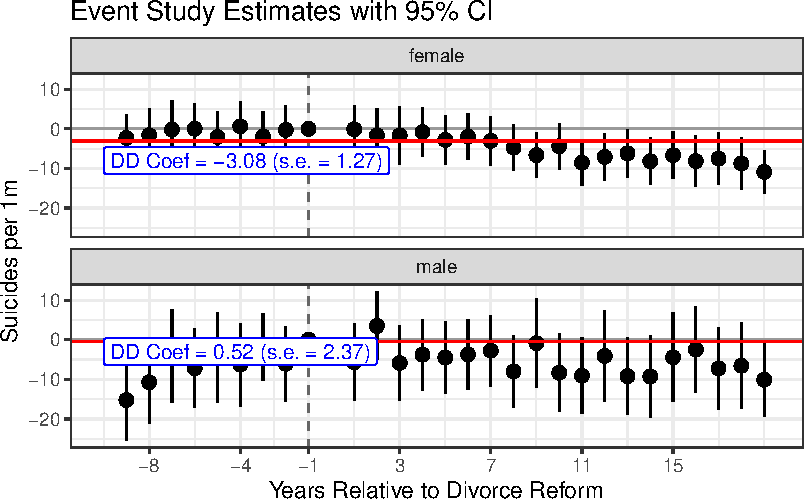
\includegraphics[keepaspectratio]{report_files/figure-pdf/unnamed-chunk-4-1.pdf}}

This event study is helpful because it shows the visual heuristics in
determining the credibility of the parallel trends. When we look at the
pre-trends of the outcomes, we can see that the outcome differences are
insignificant. Since this is at least true to female outcome, it
supports the paper's claim of parallel trends assumption. The event
study is also helpful in examining some dynamic effects of the outcome
of interest over time. We can see that the negative effects on female
suicidal rates are mostly driven from effects after 7 years of the
policy change.

\subsection{Q5}\label{q5}

Remember that generalized D-D model averages together following types of
effects:

\begin{enumerate}
\def\labelenumi{\arabic{enumi}.}
\item
  groups that are treated late vs groups that are treated early
\item
  groups that are treated early vs groups that are treated late
\item
  groups that are always treated vs groups that are treated at some
  point in the sample period
\item
  groups that are never treated vs groups that are treated at some point
  in the sample period
\end{enumerate}

TWFE estimates can be biased in a staggered adoption setting because
effects for some of these groups may receive negative weights. using
CH2020 notation, the weights are defined as:

\[
 w_{fe,g,t} = \frac{\varepsilon_{fe,g,t}}{\sum_{(g,t): D_{g,t}=1} \frac{N_{g,t}}{N_1} \varepsilon_{fe,g,t}}
\]

where \(\varepsilon\) is the residual of the observations in \((g,t)\)
cell from the regression of treatment indicator \(D\). You can see that
the weights can be negative as \(\varepsilon\) can be negative.
According to CH2020, when treatment effects are dynamic and/or
heterogeneous, average outcomes across groups may follow different tends
across periods, leading to negative weights. Usually groups that stay
treated for more periods and periods where a large number of groups are
treated are more likely to have negative weights.

\subsection{Q6}\label{q6}

We now produce alternate versions of the event study using
Callaway-Santanna and the BJS imputation estimators. Note that we only
do the result for female. First, we give you the event study plot for
BJS (2021):

\begin{Shaded}
\begin{Highlighting}[]
\FunctionTok{library}\NormalTok{(did2s)}

\NormalTok{data\_al }\OtherTok{\textless{}{-}}\NormalTok{ data }\SpecialCharTok{\%\textgreater{}\%} 
  \FunctionTok{filter}\NormalTok{(nfd }\SpecialCharTok{!=} \StringTok{"PRE"}\NormalTok{) }\SpecialCharTok{\%\textgreater{}\%} 
  \FunctionTok{mutate}\NormalTok{(}\AttributeTok{g =} \FunctionTok{ifelse}\NormalTok{(nfd }\SpecialCharTok{==} \StringTok{"NRS"}\NormalTok{, }\ConstantTok{NA}\NormalTok{, nfd))}

\NormalTok{multiple\_ests\_w }\OtherTok{=}\NormalTok{ did2s}\SpecialCharTok{::}\FunctionTok{event\_study}\NormalTok{(}
  \AttributeTok{data =}\NormalTok{ data\_al }\SpecialCharTok{\%\textgreater{}\%} 
    \FunctionTok{mutate}\NormalTok{(}\AttributeTok{asmrs =}\NormalTok{ asmrs }\SpecialCharTok{*} \DecValTok{10}\NormalTok{, }\AttributeTok{g =} \FunctionTok{as.numeric}\NormalTok{(g)) }\SpecialCharTok{\%\textgreater{}\%} 
    \FunctionTok{filter}\NormalTok{(sex}\SpecialCharTok{==}\DecValTok{2}\NormalTok{),}
  \AttributeTok{gname =} \StringTok{"g"}\NormalTok{,}
  \AttributeTok{idname =} \StringTok{"stfips"}\NormalTok{,}
  \AttributeTok{tname =} \StringTok{"year"}\NormalTok{,}
  \AttributeTok{yname =} \StringTok{"asmrs"}\NormalTok{,}
  \AttributeTok{estimator =} \StringTok{"impute"}
\NormalTok{)}

\FunctionTok{plot\_event\_study}\NormalTok{(multiple\_ests\_w)}
\end{Highlighting}
\end{Shaded}

\pandocbounded{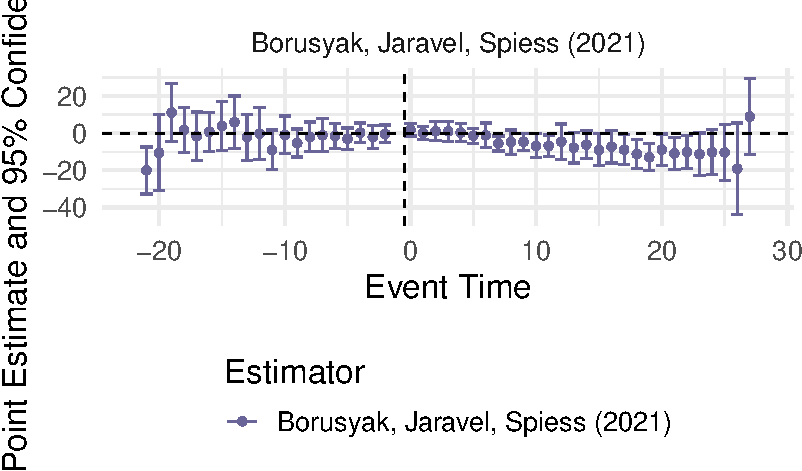
\includegraphics[keepaspectratio]{report_files/figure-pdf/unnamed-chunk-5-1.pdf}}

Next is CS (2020):

\begin{Shaded}
\begin{Highlighting}[]
\NormalTok{multiple\_ests\_w }\OtherTok{=}\NormalTok{ did2s}\SpecialCharTok{::}\FunctionTok{event\_study}\NormalTok{(}
  \AttributeTok{data =}\NormalTok{ data\_al }\SpecialCharTok{\%\textgreater{}\%} 
    \FunctionTok{mutate}\NormalTok{(}\AttributeTok{asmrs =}\NormalTok{ asmrs }\SpecialCharTok{*} \DecValTok{10}\NormalTok{, }\AttributeTok{g =} \FunctionTok{as.numeric}\NormalTok{(g)) }\SpecialCharTok{\%\textgreater{}\%} 
    \FunctionTok{filter}\NormalTok{(sex}\SpecialCharTok{==}\DecValTok{2}\NormalTok{),}
  \AttributeTok{gname =} \StringTok{"g"}\NormalTok{,}
  \AttributeTok{idname =} \StringTok{"stfips"}\NormalTok{,}
  \AttributeTok{tname =} \StringTok{"year"}\NormalTok{,}
  \AttributeTok{yname =} \StringTok{"asmrs"}\NormalTok{,}
  \AttributeTok{estimator =} \StringTok{"did"}
\NormalTok{)}

\FunctionTok{plot\_event\_study}\NormalTok{(multiple\_ests\_w)}
\end{Highlighting}
\end{Shaded}

\pandocbounded{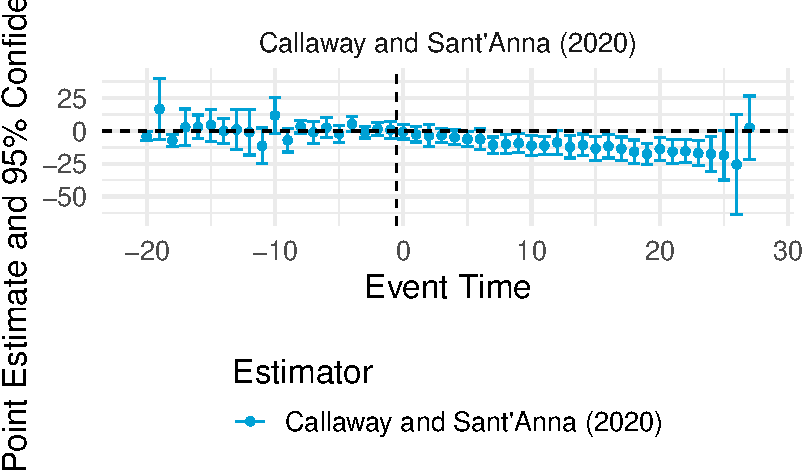
\includegraphics[keepaspectratio]{report_files/figure-pdf/unnamed-chunk-6-1.pdf}}

It seems the result is qualitatively similar to the results in the past
paper. That is, we can still see the downward trend after the change in
the divorce law. However, the overall dynamic effects seem to be less
significant than the results in the past paper. As we mentioned in Q5,
this difference might be due to the negative weighting problem. As TWFE
also does forbidden comparison between treatment groups and groups that
were already treated in the past, the results could be partially biased.

But it is important to note that the effect still seems to exist: After
the policy shock, the suicidal rates of female seem to decrease.

\subsection{Q7}\label{q7}

Now we will replicate Figure 6 in GB2021 using the bacondecomp command.
We will but first compute the weights assigned to different categories
of estimators:

\begin{Shaded}
\begin{Highlighting}[]
\FunctionTok{library}\NormalTok{(bacondecomp)}

\NormalTok{data }\OtherTok{\textless{}{-}}\NormalTok{ data }\SpecialCharTok{\%\textgreater{}\%} \FunctionTok{mutate}\NormalTok{(}\AttributeTok{asm =}\NormalTok{ asmrs }\SpecialCharTok{*} \DecValTok{10}\NormalTok{)}

\NormalTok{df\_bacon }\OtherTok{\textless{}{-}} \FunctionTok{bacon}\NormalTok{(asm }\SpecialCharTok{\textasciitilde{}}\NormalTok{ post,}
            \AttributeTok{data =}\NormalTok{ data,}
            \AttributeTok{id\_var =} \StringTok{"stfips"}\NormalTok{,}
            \AttributeTok{time\_var =} \StringTok{"year"}\NormalTok{)}
\end{Highlighting}
\end{Shaded}

\begin{verbatim}
                      type  weight  avg_est
1 Earlier vs Later Treated 0.11065 -3.57476
2  Later vs Always Treated 0.38443 -2.49401
3 Later vs Earlier Treated 0.26464  4.91700
4     Treated vs Untreated 0.24027 -5.10410
\end{verbatim}

\begin{Shaded}
\begin{Highlighting}[]
\FunctionTok{ggplot}\NormalTok{(df\_bacon) }\SpecialCharTok{+}
  \FunctionTok{aes}\NormalTok{(}\AttributeTok{x =}\NormalTok{ weight, }\AttributeTok{y =}\NormalTok{ estimate, }\AttributeTok{shape =} \FunctionTok{factor}\NormalTok{(type))}\SpecialCharTok{+}
  \FunctionTok{labs}\NormalTok{(}\AttributeTok{x=}\StringTok{"Weight"}\NormalTok{, }\AttributeTok{y =} \StringTok{"2x2 DD Estimate"}\NormalTok{, }\AttributeTok{shape =} \StringTok{"Type"}\NormalTok{) }\SpecialCharTok{+}
  \FunctionTok{geom\_point}\NormalTok{() }\SpecialCharTok{+}
  \FunctionTok{geom\_hline}\NormalTok{(}\AttributeTok{yintercept=}\SpecialCharTok{{-}}\FloatTok{3.08}\NormalTok{, }\AttributeTok{colour =} \StringTok{"red"}\NormalTok{) }\SpecialCharTok{+}
  \FunctionTok{theme\_bw}\NormalTok{()}
\end{Highlighting}
\end{Shaded}

\pandocbounded{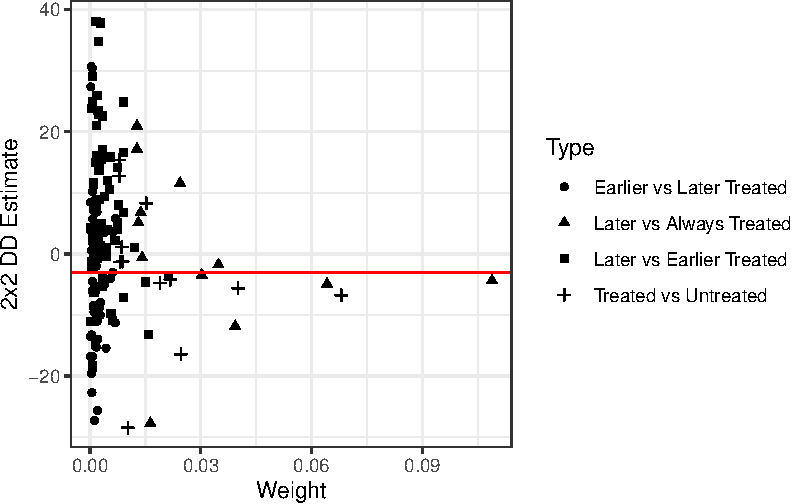
\includegraphics[keepaspectratio]{report_files/figure-pdf/unnamed-chunk-7-1.pdf}}

Note that the weights are positive for all categories. It seems Earlier
vs later cateogry have the lowest weights. Also the only positive
average estimates is in later vs earlier treated category. Since is has
a weight 0.26, this estimate will be shifting the overall estimate
upward toward 0, possibly leading to bias.

\section{Sant'anna simulations}\label{santanna-simulations}

We can just use and follow the codes given by Sant'anna. Using it, we
can get a plot similar to his figure:

\subsection{Q1}\label{q1-1}

\begin{Shaded}
\begin{Highlighting}[]
\FunctionTok{library}\NormalTok{(did) }
\FunctionTok{library}\NormalTok{(lfe)}
\FunctionTok{library}\NormalTok{(fastDummies)}
\FunctionTok{library}\NormalTok{(ggthemes)}
\FunctionTok{theme\_set}\NormalTok{(}\FunctionTok{theme\_clean}\NormalTok{() }\SpecialCharTok{+} \FunctionTok{theme}\NormalTok{(}\AttributeTok{plot.background =} \FunctionTok{element\_blank}\NormalTok{()))}

\NormalTok{iseed }\OtherTok{=} \DecValTok{20201221}
\NormalTok{nrep }\OtherTok{\textless{}{-}} \DecValTok{100}
\NormalTok{true\_mu }\OtherTok{\textless{}{-}} \DecValTok{1}
\FunctionTok{set.seed}\NormalTok{(iseed)}

\DocumentationTok{\#\# Generate data {-} treated cohorts consist of 250 obs each, with the treatment effect still = true\_mu on average}
\NormalTok{make\_data3 }\OtherTok{\textless{}{-}} \ControlFlowTok{function}\NormalTok{(}\AttributeTok{nobs =} \DecValTok{1000}\NormalTok{, }
                      \AttributeTok{nstates =} \DecValTok{40}\NormalTok{) \{}
  
  \CommentTok{\# unit fixed effects (unobservd heterogeneity)}
\NormalTok{  unit }\OtherTok{\textless{}{-}} \FunctionTok{tibble}\NormalTok{(}
    \AttributeTok{unit =} \DecValTok{1}\SpecialCharTok{:}\NormalTok{nobs,}
    \CommentTok{\# generate state}
    \AttributeTok{state =} \FunctionTok{sample}\NormalTok{(}\DecValTok{1}\SpecialCharTok{:}\NormalTok{nstates, nobs, }\AttributeTok{replace =} \ConstantTok{TRUE}\NormalTok{),}
    \AttributeTok{unit\_fe =} \FunctionTok{rnorm}\NormalTok{(nobs, state}\SpecialCharTok{/}\DecValTok{5}\NormalTok{, }\DecValTok{1}\NormalTok{),}
    \CommentTok{\# generate instantaneous treatment effect}
    \CommentTok{\#mu = rnorm(nobs, true\_mu, 0.2)}
    \AttributeTok{mu =}\NormalTok{ true\_mu}
\NormalTok{  )}
  
  \CommentTok{\# year fixed effects (first part)}
\NormalTok{  year }\OtherTok{\textless{}{-}} \FunctionTok{tibble}\NormalTok{(}
    \AttributeTok{year =} \DecValTok{1980}\SpecialCharTok{:}\DecValTok{2010}\NormalTok{,}
    \AttributeTok{year\_fe =} \FunctionTok{rnorm}\NormalTok{(}\FunctionTok{length}\NormalTok{(year), }\DecValTok{0}\NormalTok{, }\DecValTok{1}\NormalTok{)}
\NormalTok{  )}
  
  \CommentTok{\# Put the states into treatment groups}
\NormalTok{  treat\_taus }\OtherTok{\textless{}{-}} \FunctionTok{tibble}\NormalTok{(}
    \CommentTok{\# sample the states randomly}
    \AttributeTok{state =} \FunctionTok{sample}\NormalTok{(}\DecValTok{1}\SpecialCharTok{:}\NormalTok{nstates, nstates, }\AttributeTok{replace =} \ConstantTok{FALSE}\NormalTok{),}
    \CommentTok{\# place the randomly sampled states into 1\textbackslash{}\{t \textbackslash{}ge g \textbackslash{}\}G\_g}
    \AttributeTok{cohort\_year =} \FunctionTok{sort}\NormalTok{(}\FunctionTok{rep}\NormalTok{(}\FunctionTok{c}\NormalTok{(}\DecValTok{1986}\NormalTok{, }\DecValTok{1992}\NormalTok{, }\DecValTok{1998}\NormalTok{, }\DecValTok{2004}\NormalTok{), }\DecValTok{10}\NormalTok{))}
\NormalTok{  )}
  
  \CommentTok{\# make main dataset}
  \CommentTok{\# full interaction of unit X year }
  \FunctionTok{expand\_grid}\NormalTok{(}\AttributeTok{unit =} \DecValTok{1}\SpecialCharTok{:}\NormalTok{nobs, }\AttributeTok{year =} \DecValTok{1980}\SpecialCharTok{:}\DecValTok{2010}\NormalTok{) }\SpecialCharTok{\%\textgreater{}\%} 
    \FunctionTok{left\_join}\NormalTok{(., unit) }\SpecialCharTok{\%\textgreater{}\%} 
    \FunctionTok{left\_join}\NormalTok{(., year) }\SpecialCharTok{\%\textgreater{}\%} 
    \FunctionTok{left\_join}\NormalTok{(., treat\_taus) }\SpecialCharTok{\%\textgreater{}\%} 
    \CommentTok{\# make error term and get treatment indicators and treatment effects}
    \CommentTok{\# Also get cohort specific trends (modify time FE)}
    \FunctionTok{mutate}\NormalTok{(}\AttributeTok{error =} \FunctionTok{rnorm}\NormalTok{(nobs}\SpecialCharTok{*}\DecValTok{31}\NormalTok{, }\DecValTok{0}\NormalTok{, }\DecValTok{1}\NormalTok{),}
           \AttributeTok{treat =} \FunctionTok{ifelse}\NormalTok{((year }\SpecialCharTok{\textgreater{}=}\NormalTok{ cohort\_year)}\SpecialCharTok{*}\NormalTok{ (cohort\_year }\SpecialCharTok{!=} \DecValTok{2004}\NormalTok{), }\DecValTok{1}\NormalTok{, }\DecValTok{0}\NormalTok{),}
           \AttributeTok{mu =} \FunctionTok{ifelse}\NormalTok{(cohort\_year}\SpecialCharTok{==}\DecValTok{1992}\NormalTok{, }\DecValTok{2}\NormalTok{, }\FunctionTok{ifelse}\NormalTok{(cohort\_year}\SpecialCharTok{==}\DecValTok{1998}\NormalTok{, }\DecValTok{1}\NormalTok{, }\DecValTok{3}\NormalTok{)),}
           \AttributeTok{tau =} \FunctionTok{ifelse}\NormalTok{(treat }\SpecialCharTok{==} \DecValTok{1}\NormalTok{, mu, }\DecValTok{0}\NormalTok{),}
           \AttributeTok{year\_fe =}\NormalTok{ year\_fe }\SpecialCharTok{+} \FloatTok{0.1}\SpecialCharTok{*}\NormalTok{(year }\SpecialCharTok{{-}}\NormalTok{ cohort\_year)}
\NormalTok{    ) }\SpecialCharTok{\%\textgreater{}\%} 
    \CommentTok{\# calculate cumulative treatment effects}
    \FunctionTok{group\_by}\NormalTok{(unit) }\SpecialCharTok{\%\textgreater{}\%} 
    \FunctionTok{mutate}\NormalTok{(}\AttributeTok{tau\_cum =} \FunctionTok{cumsum}\NormalTok{(tau)) }\SpecialCharTok{\%\textgreater{}\%} 
    \FunctionTok{ungroup}\NormalTok{() }\SpecialCharTok{\%\textgreater{}\%} 
    \CommentTok{\# calculate the dep variable}
    \FunctionTok{mutate}\NormalTok{(}\AttributeTok{dep\_var =}\NormalTok{ (}\DecValTok{2010} \SpecialCharTok{{-}}\NormalTok{ cohort\_year) }\SpecialCharTok{+}\NormalTok{ unit\_fe }\SpecialCharTok{+}\NormalTok{ year\_fe }\SpecialCharTok{+}\NormalTok{ tau\_cum }\SpecialCharTok{+}\NormalTok{ error) }\SpecialCharTok{\%\textgreater{}\%}
    \CommentTok{\# Relabel 2004 cohort as never{-}treated}
    \FunctionTok{mutate}\NormalTok{(}\AttributeTok{cohort\_year =} \FunctionTok{ifelse}\NormalTok{(cohort\_year }\SpecialCharTok{==} \DecValTok{2004}\NormalTok{, }\ConstantTok{Inf}\NormalTok{, cohort\_year))}
  
\NormalTok{\}}
\CommentTok{\#{-}{-}{-}{-}{-}{-}{-}{-}{-}{-}{-}{-}{-}{-}{-}{-}{-}{-}{-}{-}{-}{-}{-}{-}{-}{-}{-}{-}{-}{-}{-}{-}{-}{-}{-}{-}{-}{-}{-}{-}{-}{-}{-}{-}{-}{-}{-}{-}{-}{-}{-}{-}{-}{-}{-}{-}{-}{-}{-}{-}{-}{-}{-}{-}{-}{-}{-}{-}{-}{-}{-}{-}{-}{-}{-}{-}}
\CommentTok{\# make data}
\NormalTok{data }\OtherTok{\textless{}{-}} \FunctionTok{make\_data3}\NormalTok{()}

\CommentTok{\# plot}
\NormalTok{plot3 }\OtherTok{\textless{}{-}}\NormalTok{ data }\SpecialCharTok{\%\textgreater{}\%} 
  \FunctionTok{ggplot}\NormalTok{(}\FunctionTok{aes}\NormalTok{(}\AttributeTok{x =}\NormalTok{ year, }\AttributeTok{y =}\NormalTok{ dep\_var, }\AttributeTok{group =}\NormalTok{ unit)) }\SpecialCharTok{+} 
  \FunctionTok{geom\_line}\NormalTok{(}\AttributeTok{alpha =} \DecValTok{1}\SpecialCharTok{/}\DecValTok{8}\NormalTok{, }\AttributeTok{color =} \StringTok{"grey"}\NormalTok{) }\SpecialCharTok{+} 
  \FunctionTok{geom\_line}\NormalTok{(}\AttributeTok{data =}\NormalTok{ data }\SpecialCharTok{\%\textgreater{}\%} 
              \FunctionTok{group\_by}\NormalTok{(cohort\_year, year) }\SpecialCharTok{\%\textgreater{}\%} 
              \FunctionTok{summarize}\NormalTok{(}\AttributeTok{dep\_var =} \FunctionTok{mean}\NormalTok{(dep\_var)),}
            \FunctionTok{aes}\NormalTok{(}\AttributeTok{x =}\NormalTok{ year, }\AttributeTok{y =}\NormalTok{ dep\_var, }\AttributeTok{group =} \FunctionTok{factor}\NormalTok{(cohort\_year),}
                \AttributeTok{color =} \FunctionTok{factor}\NormalTok{(cohort\_year)),}
            \AttributeTok{size =} \DecValTok{2}\NormalTok{) }\SpecialCharTok{+} 
  \FunctionTok{labs}\NormalTok{(}\AttributeTok{x =} \StringTok{""}\NormalTok{, }\AttributeTok{y =} \StringTok{"Value"}\NormalTok{,  }\AttributeTok{color =} \StringTok{"Treatment group   "}\NormalTok{) }\SpecialCharTok{+} 
  \FunctionTok{geom\_vline}\NormalTok{(}\AttributeTok{xintercept =} \DecValTok{1986}\NormalTok{, }\AttributeTok{color =} \StringTok{\textquotesingle{}\#E41A1C\textquotesingle{}}\NormalTok{, }\AttributeTok{size =} \DecValTok{2}\NormalTok{) }\SpecialCharTok{+} 
  \FunctionTok{geom\_vline}\NormalTok{(}\AttributeTok{xintercept =} \DecValTok{1992}\NormalTok{, }\AttributeTok{color =} \StringTok{\textquotesingle{}\#377EB8\textquotesingle{}}\NormalTok{, }\AttributeTok{size =} \DecValTok{2}\NormalTok{) }\SpecialCharTok{+} 
  \FunctionTok{geom\_vline}\NormalTok{(}\AttributeTok{xintercept =} \DecValTok{1998}\NormalTok{, }\AttributeTok{color =} \StringTok{\textquotesingle{}\#4DAF4A\textquotesingle{}}\NormalTok{, }\AttributeTok{size =} \DecValTok{2}\NormalTok{) }\SpecialCharTok{+} 
  \CommentTok{\#geom\_vline(xintercept = 2004, color = \textquotesingle{}\#984EA3\textquotesingle{}, size = 2) + }
  \FunctionTok{scale\_color\_brewer}\NormalTok{(}\AttributeTok{palette =} \StringTok{\textquotesingle{}Set1\textquotesingle{}}\NormalTok{) }\SpecialCharTok{+} 
  \FunctionTok{theme}\NormalTok{(}\AttributeTok{legend.position =} \StringTok{\textquotesingle{}bottom\textquotesingle{}}\NormalTok{,}
        \CommentTok{\#legend.title = element\_blank(), }
        \AttributeTok{axis.title =} \FunctionTok{element\_text}\NormalTok{(}\AttributeTok{size =} \DecValTok{14}\NormalTok{),}
        \AttributeTok{axis.text =} \FunctionTok{element\_text}\NormalTok{(}\AttributeTok{size =} \DecValTok{12}\NormalTok{)) }\SpecialCharTok{+}
  \FunctionTok{scale\_color\_manual}\NormalTok{(}\AttributeTok{labels =} \FunctionTok{c}\NormalTok{(}\StringTok{"1986"}\NormalTok{, }\StringTok{"1992"}\NormalTok{, }\StringTok{"1998"}\NormalTok{, }\StringTok{"Never{-}treated"}\NormalTok{),}
                     \AttributeTok{values =} \FunctionTok{c}\NormalTok{(}\StringTok{"\#E41A1C"}\NormalTok{, }\StringTok{"\#377EB8"}\NormalTok{, }\StringTok{"\#4DAF4A"}\NormalTok{, }\StringTok{"\#984EA3"}\NormalTok{)) }\SpecialCharTok{+}
  \FunctionTok{ggtitle}\NormalTok{(}\StringTok{"One draw of the DGP with heterogeneous treatment effect dynamics across cohorts }\SpecialCharTok{\textbackslash{}n}\StringTok{ and with a never{-}treated group"}\NormalTok{)}\SpecialCharTok{+}
  \FunctionTok{theme}\NormalTok{(}\AttributeTok{plot.title =} \FunctionTok{element\_text}\NormalTok{(}\AttributeTok{hjust =} \FloatTok{0.5}\NormalTok{, }\AttributeTok{size=}\DecValTok{12}\NormalTok{))}

\NormalTok{plot3 }
\end{Highlighting}
\end{Shaded}

\pandocbounded{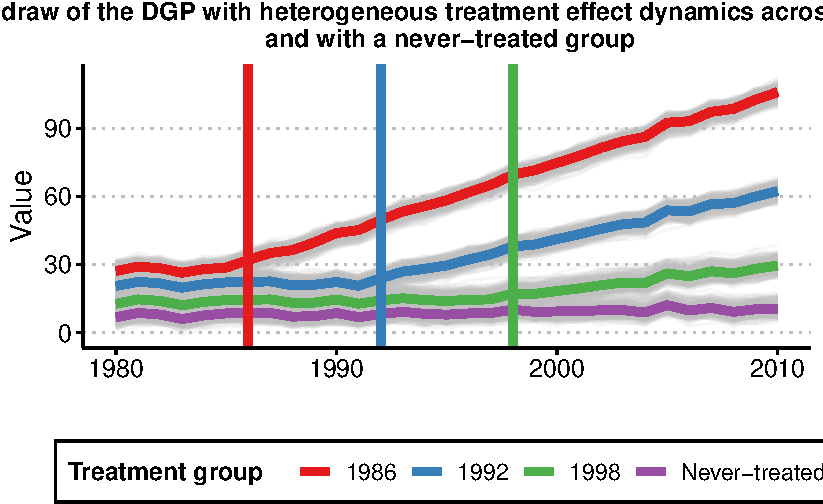
\includegraphics[keepaspectratio]{report_files/figure-pdf/unnamed-chunk-8-1.pdf}}

\subsection{Q2}\label{q2-1}

We can see that the TWFE estimator is biased downwards. Thus, the
estimator does not retrieve the true treatment effects.

\begin{Shaded}
\begin{Highlighting}[]
\CommentTok{\# function to run ES DID}
\NormalTok{run\_ES\_DiD\_sat\_never\_het }\OtherTok{\textless{}{-}} \ControlFlowTok{function}\NormalTok{(...) \{}
  
  \CommentTok{\# resimulate the data}
\NormalTok{  data }\OtherTok{\textless{}{-}} \FunctionTok{make\_data3}\NormalTok{()}
  
  \CommentTok{\# make dummy columns}
\NormalTok{  data }\OtherTok{\textless{}{-}}\NormalTok{ data }\SpecialCharTok{\%\textgreater{}\%} 
    \CommentTok{\# make relative year indicator}
    \FunctionTok{mutate}\NormalTok{(}\AttributeTok{rel\_year =}\NormalTok{ year }\SpecialCharTok{{-}}\NormalTok{ cohort\_year)}
  
  \CommentTok{\# get the minimum relative year {-} we need this to reindex}
\NormalTok{  min\_year }\OtherTok{\textless{}{-}} \FunctionTok{min}\NormalTok{(data}\SpecialCharTok{$}\NormalTok{rel\_year }\SpecialCharTok{*}\NormalTok{ (data}\SpecialCharTok{$}\NormalTok{rel\_year }\SpecialCharTok{!=} \SpecialCharTok{{-}}\ConstantTok{Inf}\NormalTok{), }\AttributeTok{na.rm =}\NormalTok{ T)}
  
  \CommentTok{\# reindex the relative years}
\NormalTok{  data }\OtherTok{\textless{}{-}}\NormalTok{ data }\SpecialCharTok{\%\textgreater{}\%} 
    \FunctionTok{mutate}\NormalTok{(}\AttributeTok{rel\_year2 =}\NormalTok{ rel\_year) }\SpecialCharTok{\%\textgreater{}\%} 
    \FunctionTok{mutate}\NormalTok{(}\AttributeTok{rel\_year =}\NormalTok{ rel\_year }\SpecialCharTok{{-}}\NormalTok{ min\_year) }\SpecialCharTok{\%\textgreater{}\%} 
    \FunctionTok{dummy\_cols}\NormalTok{(}\AttributeTok{select\_columns =} \StringTok{"rel\_year"}\NormalTok{) }\SpecialCharTok{\%\textgreater{}\%} 
    \FunctionTok{select}\NormalTok{(}\SpecialCharTok{{-}}\NormalTok{(}\StringTok{"rel\_year\_{-}Inf"}\NormalTok{))}
    
  
  \CommentTok{\# make regression formula }
\NormalTok{  indics }\OtherTok{\textless{}{-}} \FunctionTok{paste}\NormalTok{(}\StringTok{"rel\_year"}\NormalTok{, (}\DecValTok{1}\SpecialCharTok{:}\FunctionTok{max}\NormalTok{(data}\SpecialCharTok{$}\NormalTok{rel\_year))[}\SpecialCharTok{{-}}\NormalTok{(}\SpecialCharTok{{-}}\DecValTok{1} \SpecialCharTok{{-}}\NormalTok{ min\_year)], }\AttributeTok{sep =} \StringTok{"\_"}\NormalTok{, }\AttributeTok{collapse =} \StringTok{" + "}\NormalTok{)}
\NormalTok{  keepvars }\OtherTok{\textless{}{-}} \FunctionTok{paste}\NormalTok{(}\StringTok{"rel\_year"}\NormalTok{, }\FunctionTok{c}\NormalTok{(}\SpecialCharTok{{-}}\DecValTok{5}\SpecialCharTok{:{-}}\DecValTok{2}\NormalTok{, }\DecValTok{0}\SpecialCharTok{:}\DecValTok{5}\NormalTok{) }\SpecialCharTok{{-}}\NormalTok{ min\_year, }\AttributeTok{sep =} \StringTok{"\_"}\NormalTok{)  }
\NormalTok{  formula }\OtherTok{\textless{}{-}} \FunctionTok{as.formula}\NormalTok{(}\FunctionTok{paste}\NormalTok{(}\StringTok{"dep\_var \textasciitilde{}"}\NormalTok{, indics, }\StringTok{"| unit + year | 0 | state"}\NormalTok{))}
  
  \CommentTok{\# run mod}
\NormalTok{  mod }\OtherTok{\textless{}{-}} \FunctionTok{felm}\NormalTok{(formula, }\AttributeTok{data =}\NormalTok{ data, }\AttributeTok{exactDOF =} \ConstantTok{TRUE}\NormalTok{)}
  
  \CommentTok{\# grab the obs we need}
\CommentTok{\# grab the obs we need}
\NormalTok{  mod2 }\OtherTok{\textless{}{-}} \FunctionTok{tibble}\NormalTok{(}
    \AttributeTok{estimate =}\NormalTok{ mod}\SpecialCharTok{$}\NormalTok{coefficients,}
    \AttributeTok{term1 =} \FunctionTok{rownames}\NormalTok{(mod}\SpecialCharTok{$}\NormalTok{coefficients)}
\NormalTok{    )}
  
\NormalTok{ es }\OtherTok{\textless{}{-}}
\NormalTok{   mod2 }\SpecialCharTok{\%\textgreater{}\%} 
    \FunctionTok{filter}\NormalTok{(term1 }\SpecialCharTok{\%in\%}\NormalTok{ keepvars) }\SpecialCharTok{\%\textgreater{}\%} 
    \FunctionTok{mutate}\NormalTok{(}\AttributeTok{t =} \FunctionTok{c}\NormalTok{(}\SpecialCharTok{{-}}\DecValTok{5}\SpecialCharTok{:{-}}\DecValTok{2}\NormalTok{, }\DecValTok{0}\SpecialCharTok{:}\DecValTok{5}\NormalTok{)) }\SpecialCharTok{\%\textgreater{}\%} 
    \FunctionTok{select}\NormalTok{(t, estimate)}
\NormalTok{ es}
\NormalTok{\}}

\NormalTok{data\_sat\_never\_het }\OtherTok{\textless{}{-}} \FunctionTok{map\_dfr}\NormalTok{(}\DecValTok{1}\SpecialCharTok{:}\NormalTok{nrep, run\_ES\_DiD\_sat\_never\_het)}

\NormalTok{ES\_plot\_sat\_never\_het }\OtherTok{\textless{}{-}}\NormalTok{ data\_sat\_never\_het }\SpecialCharTok{\%\textgreater{}\%} 
  \FunctionTok{group\_by}\NormalTok{(t) }\SpecialCharTok{\%\textgreater{}\%} 
  \FunctionTok{summarize}\NormalTok{(}\AttributeTok{avg =} \FunctionTok{mean}\NormalTok{(estimate),}
            \AttributeTok{sd =} \FunctionTok{sd}\NormalTok{(estimate),}
            \AttributeTok{lower.ci =}\NormalTok{ avg }\SpecialCharTok{{-}} \FloatTok{1.96}\SpecialCharTok{*}\NormalTok{sd,}
            \AttributeTok{upper.ci =}\NormalTok{ avg }\SpecialCharTok{+} \FloatTok{1.96}\SpecialCharTok{*}\NormalTok{sd) }\SpecialCharTok{\%\textgreater{}\%} 
  \FunctionTok{bind\_rows}\NormalTok{(}\FunctionTok{tibble}\NormalTok{(}\AttributeTok{t =} \SpecialCharTok{{-}}\DecValTok{1}\NormalTok{, }\AttributeTok{avg =} \DecValTok{0}\NormalTok{, }\AttributeTok{sd =} \DecValTok{0}\NormalTok{, }\AttributeTok{lower.ci =} \DecValTok{0}\NormalTok{, }\AttributeTok{upper.ci =} \DecValTok{0}\NormalTok{)) }\SpecialCharTok{\%\textgreater{}\%} 
  \FunctionTok{mutate}\NormalTok{(}\AttributeTok{true\_tau =} \FunctionTok{ifelse}\NormalTok{(t }\SpecialCharTok{\textgreater{}=} \DecValTok{0}\NormalTok{, (t }\SpecialCharTok{+} \DecValTok{1}\NormalTok{)}\SpecialCharTok{*} \DecValTok{2}\NormalTok{, }\DecValTok{0}\NormalTok{)) }\SpecialCharTok{\%\textgreater{}\%} 
  \FunctionTok{ggplot}\NormalTok{(}\FunctionTok{aes}\NormalTok{(}\AttributeTok{x =}\NormalTok{ t, }\AttributeTok{y =}\NormalTok{ avg)) }\SpecialCharTok{+} 
  \CommentTok{\#geom\_linerange(aes(ymin = lower.ci, ymax = upper.ci), color = \textquotesingle{}darkgrey\textquotesingle{}, size = 2) + }
  \FunctionTok{geom\_ribbon}\NormalTok{(}\FunctionTok{aes}\NormalTok{(}\AttributeTok{ymin =}\NormalTok{ lower.ci, }\AttributeTok{ymax =}\NormalTok{ upper.ci), }\AttributeTok{color =} \StringTok{"lightgrey"}\NormalTok{, }\AttributeTok{alpha =} \FloatTok{0.2}\NormalTok{) }\SpecialCharTok{+}
  \FunctionTok{geom\_point}\NormalTok{(}\AttributeTok{color =} \StringTok{\textquotesingle{}blue\textquotesingle{}}\NormalTok{, }\AttributeTok{size =} \DecValTok{3}\NormalTok{) }\SpecialCharTok{+} 
   \FunctionTok{geom\_line}\NormalTok{(}\FunctionTok{aes}\NormalTok{(}\AttributeTok{color =} \StringTok{\textquotesingle{}Estimated Effect\textquotesingle{}}\NormalTok{), }\AttributeTok{size =} \DecValTok{1}\NormalTok{) }\SpecialCharTok{+} 
   \FunctionTok{geom\_line}\NormalTok{(}\FunctionTok{aes}\NormalTok{(}\AttributeTok{x =}\NormalTok{ t, }\AttributeTok{y =}\NormalTok{ true\_tau, }\AttributeTok{color =} \StringTok{\textquotesingle{}True Effect\textquotesingle{}}\NormalTok{), }\AttributeTok{linetype =} \StringTok{"dashed"}\NormalTok{, }\AttributeTok{size =} \DecValTok{2}\NormalTok{) }\SpecialCharTok{+} 
  \FunctionTok{geom\_hline}\NormalTok{(}\AttributeTok{yintercept =} \DecValTok{0}\NormalTok{, }\AttributeTok{linetype =} \StringTok{"dashed"}\NormalTok{) }\SpecialCharTok{+} 
  \FunctionTok{scale\_x\_continuous}\NormalTok{(}\AttributeTok{breaks =} \SpecialCharTok{{-}}\DecValTok{5}\SpecialCharTok{:}\DecValTok{5}\NormalTok{) }\SpecialCharTok{+} 
  \FunctionTok{labs}\NormalTok{(}\AttributeTok{x =} \StringTok{"Relative Time"}\NormalTok{, }\AttributeTok{y =} \StringTok{"Estimate"}\NormalTok{) }\SpecialCharTok{+} 
  \FunctionTok{theme}\NormalTok{(}\AttributeTok{axis.title =} \FunctionTok{element\_text}\NormalTok{(}\AttributeTok{size =} \DecValTok{14}\NormalTok{),}
        \AttributeTok{axis.text =} \FunctionTok{element\_text}\NormalTok{(}\AttributeTok{size =} \DecValTok{12}\NormalTok{))}\SpecialCharTok{+}
  \FunctionTok{ggtitle}\NormalTok{(}\StringTok{"TWFE event{-}study regression with \textquotesingle{}all\textquotesingle{} leads and lags"}\NormalTok{)}\SpecialCharTok{+}
  \CommentTok{\# scale\_color\_manual(values = colors) + }
  \FunctionTok{theme}\NormalTok{(}\AttributeTok{plot.title =} \FunctionTok{element\_text}\NormalTok{(}\AttributeTok{hjust =} \FloatTok{0.5}\NormalTok{, }\AttributeTok{size=}\DecValTok{12}\NormalTok{),}
        \AttributeTok{legend.position =} \StringTok{"bottom"}\NormalTok{, }
        \AttributeTok{legend.title =} \FunctionTok{element\_blank}\NormalTok{())}

\NormalTok{ES\_plot\_sat\_never\_het }
\end{Highlighting}
\end{Shaded}

\pandocbounded{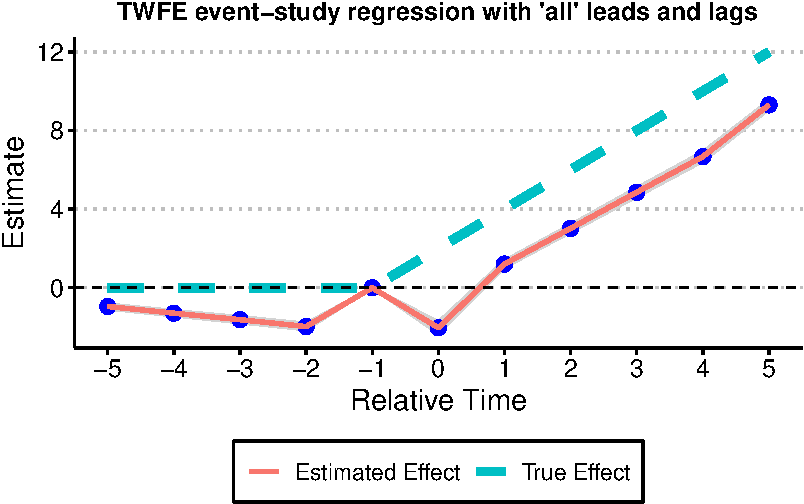
\includegraphics[keepaspectratio]{report_files/figure-pdf/unnamed-chunk-9-1.pdf}}

\subsection{Q3}\label{q3-1}

Again we use Sant'anna's code to replicate. Now it seems the esimates
match the true effects:

\begin{Shaded}
\begin{Highlighting}[]
\CommentTok{\# function to run ES DID}
\NormalTok{run\_CS\_never\_het }\OtherTok{\textless{}{-}} \ControlFlowTok{function}\NormalTok{(...) \{}
  
  \CommentTok{\# resimulate the data}
\NormalTok{  data }\OtherTok{\textless{}{-}} \FunctionTok{make\_data3}\NormalTok{()}
\NormalTok{  data}\SpecialCharTok{$}\NormalTok{cohort\_year[data}\SpecialCharTok{$}\NormalTok{cohort\_year}\SpecialCharTok{==}\ConstantTok{Inf}\NormalTok{] }\OtherTok{\textless{}{-}} \DecValTok{0}
  
\NormalTok{  mod }\OtherTok{\textless{}{-}}\NormalTok{ did}\SpecialCharTok{::}\FunctionTok{att\_gt}\NormalTok{(}\AttributeTok{yname =} \StringTok{"dep\_var"}\NormalTok{, }
                     \AttributeTok{tname =} \StringTok{"year"}\NormalTok{,}
                     \AttributeTok{idname =} \StringTok{"unit"}\NormalTok{,}
                     \AttributeTok{gname =} \StringTok{"cohort\_year"}\NormalTok{,}
                     \AttributeTok{control\_group=} \StringTok{"nevertreated"}\NormalTok{,}
                     \AttributeTok{bstrap =} \ConstantTok{FALSE}\NormalTok{,}
                     \AttributeTok{data =}\NormalTok{ data,}
                     \AttributeTok{print\_details =} \ConstantTok{FALSE}\NormalTok{)}
\NormalTok{  event\_std }\OtherTok{\textless{}{-}}\NormalTok{ did}\SpecialCharTok{::}\FunctionTok{aggte}\NormalTok{(mod, }\AttributeTok{type =} \StringTok{"dynamic"}\NormalTok{)}
  
\NormalTok{  att.egt }\OtherTok{\textless{}{-}}\NormalTok{ event\_std}\SpecialCharTok{$}\NormalTok{att.egt}
  \FunctionTok{names}\NormalTok{(att.egt) }\OtherTok{\textless{}{-}}\NormalTok{ event\_std}\SpecialCharTok{$}\NormalTok{egt}
  
  \CommentTok{\# grab the obs we need}
\NormalTok{  broom}\SpecialCharTok{::}\FunctionTok{tidy}\NormalTok{(att.egt) }\SpecialCharTok{\%\textgreater{}\%} 
    \FunctionTok{filter}\NormalTok{(names }\SpecialCharTok{\%in\%} \SpecialCharTok{{-}}\DecValTok{5}\SpecialCharTok{:}\DecValTok{5}\NormalTok{) }\SpecialCharTok{\%\textgreater{}\%} 
    \FunctionTok{mutate}\NormalTok{(}\AttributeTok{t =} \SpecialCharTok{{-}}\DecValTok{5}\SpecialCharTok{:}\DecValTok{5}\NormalTok{, }\AttributeTok{estimate =}\NormalTok{ x) }\SpecialCharTok{\%\textgreater{}\%} 
    \FunctionTok{select}\NormalTok{(t, estimate)}
\NormalTok{\}}

\NormalTok{data\_CS\_never\_het }\OtherTok{\textless{}{-}} \FunctionTok{map\_dfr}\NormalTok{(}\DecValTok{1}\SpecialCharTok{:}\NormalTok{nrep, run\_CS\_never\_het)}

\NormalTok{ES\_plot\_CS\_never\_het }\OtherTok{\textless{}{-}}\NormalTok{ data\_CS\_never\_het }\SpecialCharTok{\%\textgreater{}\%} 
  \FunctionTok{group\_by}\NormalTok{(t) }\SpecialCharTok{\%\textgreater{}\%} 
  \FunctionTok{summarize}\NormalTok{(}\AttributeTok{avg =} \FunctionTok{mean}\NormalTok{(estimate),}
            \AttributeTok{sd =} \FunctionTok{sd}\NormalTok{(estimate),}
            \AttributeTok{lower.ci =}\NormalTok{ avg }\SpecialCharTok{{-}} \FloatTok{1.96}\SpecialCharTok{*}\NormalTok{sd,}
            \AttributeTok{upper.ci =}\NormalTok{ avg }\SpecialCharTok{+} \FloatTok{1.96}\SpecialCharTok{*}\NormalTok{sd) }\SpecialCharTok{\%\textgreater{}\%} 
  \FunctionTok{mutate}\NormalTok{(}\AttributeTok{true\_tau =} \FunctionTok{ifelse}\NormalTok{(t }\SpecialCharTok{\textgreater{}=} \DecValTok{0}\NormalTok{, (t }\SpecialCharTok{+} \DecValTok{1}\NormalTok{)}\SpecialCharTok{*} \DecValTok{2}\NormalTok{, }\DecValTok{0}\NormalTok{)) }\SpecialCharTok{\%\textgreater{}\%} 
  \FunctionTok{ggplot}\NormalTok{(}\FunctionTok{aes}\NormalTok{(}\AttributeTok{x =}\NormalTok{ t, }\AttributeTok{y =}\NormalTok{ avg)) }\SpecialCharTok{+} 
  \CommentTok{\#geom\_linerange(aes(ymin = lower.ci, ymax = upper.ci), color = \textquotesingle{}darkgrey\textquotesingle{}, size = 2) + }
  \FunctionTok{geom\_ribbon}\NormalTok{(}\FunctionTok{aes}\NormalTok{(}\AttributeTok{ymin =}\NormalTok{ lower.ci, }\AttributeTok{ymax =}\NormalTok{ upper.ci), }\AttributeTok{color =} \StringTok{"lightgrey"}\NormalTok{, }\AttributeTok{alpha =} \FloatTok{0.2}\NormalTok{) }\SpecialCharTok{+}
  \FunctionTok{geom\_point}\NormalTok{(}\AttributeTok{color =} \StringTok{\textquotesingle{}blue\textquotesingle{}}\NormalTok{, }\AttributeTok{size =} \DecValTok{3}\NormalTok{) }\SpecialCharTok{+} 
   \FunctionTok{geom\_line}\NormalTok{(}\FunctionTok{aes}\NormalTok{(}\AttributeTok{color =} \StringTok{\textquotesingle{}Estimated Effect\textquotesingle{}}\NormalTok{), }\AttributeTok{size =} \DecValTok{1}\NormalTok{) }\SpecialCharTok{+} 
   \FunctionTok{geom\_line}\NormalTok{(}\FunctionTok{aes}\NormalTok{(}\AttributeTok{x =}\NormalTok{ t, }\AttributeTok{y =}\NormalTok{ true\_tau, }\AttributeTok{color =} \StringTok{\textquotesingle{}True Effect\textquotesingle{}}\NormalTok{), }\AttributeTok{linetype =} \StringTok{"dashed"}\NormalTok{, }\AttributeTok{size =} \DecValTok{2}\NormalTok{) }\SpecialCharTok{+} 
  \FunctionTok{geom\_hline}\NormalTok{(}\AttributeTok{yintercept =} \DecValTok{0}\NormalTok{, }\AttributeTok{linetype =} \StringTok{"dashed"}\NormalTok{) }\SpecialCharTok{+} 
  \FunctionTok{scale\_x\_continuous}\NormalTok{(}\AttributeTok{breaks =} \SpecialCharTok{{-}}\DecValTok{5}\SpecialCharTok{:}\DecValTok{5}\NormalTok{) }\SpecialCharTok{+} 
  \FunctionTok{labs}\NormalTok{(}\AttributeTok{x =} \StringTok{"Relative Time"}\NormalTok{, }\AttributeTok{y =} \StringTok{"Estimate"}\NormalTok{) }\SpecialCharTok{+} 
  \FunctionTok{theme}\NormalTok{(}\AttributeTok{axis.title =} \FunctionTok{element\_text}\NormalTok{(}\AttributeTok{size =} \DecValTok{14}\NormalTok{),}
        \AttributeTok{axis.text =} \FunctionTok{element\_text}\NormalTok{(}\AttributeTok{size =} \DecValTok{12}\NormalTok{))}\SpecialCharTok{+}
  \FunctionTok{ggtitle}\NormalTok{(}\StringTok{"Event{-}study{-}parameters estimated using Callaway and Sant\textquotesingle{}Anna (2020)}\SpecialCharTok{\textbackslash{}n}\StringTok{Comparison group: Never{-}treated units"}\NormalTok{)}\SpecialCharTok{+}
  \CommentTok{\# scale\_color\_manual(values = colors) + }
  \FunctionTok{theme}\NormalTok{(}\AttributeTok{plot.title =} \FunctionTok{element\_text}\NormalTok{(}\AttributeTok{hjust =} \FloatTok{0.5}\NormalTok{, }\AttributeTok{size=}\DecValTok{12}\NormalTok{),}
        \AttributeTok{legend.position =} \StringTok{"bottom"}\NormalTok{, }
        \AttributeTok{legend.title =} \FunctionTok{element\_blank}\NormalTok{())}

\NormalTok{ES\_plot\_CS\_never\_het}
\end{Highlighting}
\end{Shaded}

\pandocbounded{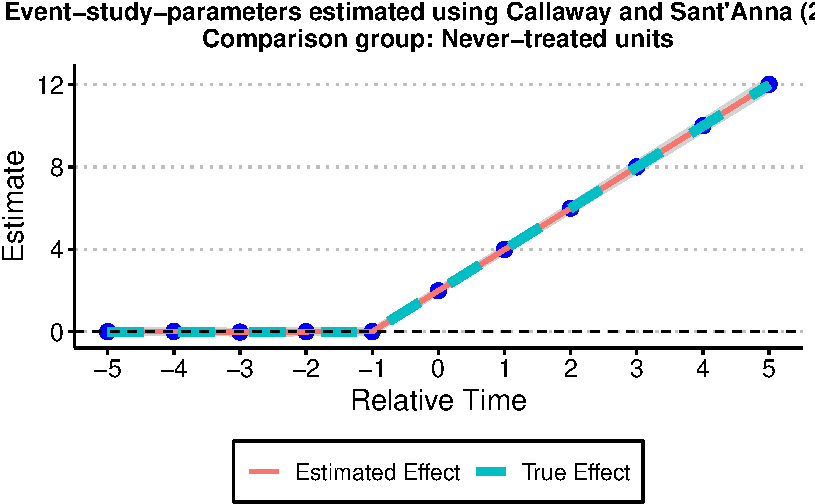
\includegraphics[keepaspectratio]{report_files/figure-pdf/unnamed-chunk-10-1.pdf}}

\subsection{Q4}\label{q4-1}

In this case, estimates of TWFE will do good job in retrieving the true
effects.

\begin{Shaded}
\begin{Highlighting}[]
\DocumentationTok{\#\# Generate data {-} treated cohorts consist of 250 obs each, with the treatment effect still = true\_mu on average}

\NormalTok{make\_data4 }\OtherTok{\textless{}{-}} \ControlFlowTok{function}\NormalTok{(}\AttributeTok{nobs =} \DecValTok{1000}\NormalTok{,}

                       \AttributeTok{nstates =} \DecValTok{40}\NormalTok{) \{}

 

  \CommentTok{\# unit fixed effects (unobservd heterogeneity)}

\NormalTok{  unit }\OtherTok{\textless{}{-}} \FunctionTok{tibble}\NormalTok{(}

    \AttributeTok{unit =} \DecValTok{1}\SpecialCharTok{:}\NormalTok{nobs,}

    \CommentTok{\# generate state}

    \AttributeTok{state =} \FunctionTok{sample}\NormalTok{(}\DecValTok{1}\SpecialCharTok{:}\NormalTok{nstates, nobs, }\AttributeTok{replace =} \ConstantTok{TRUE}\NormalTok{),}

    \AttributeTok{unit\_fe =} \FunctionTok{rnorm}\NormalTok{(nobs, state}\SpecialCharTok{/}\DecValTok{5}\NormalTok{, }\DecValTok{1}\NormalTok{),}

    \CommentTok{\# generate instantaneous treatment effect}

    \CommentTok{\#mu = rnorm(nobs, true\_mu, 0.2)}

    \AttributeTok{mu =}\NormalTok{ true\_mu}

\NormalTok{  )}

 

  \CommentTok{\# year fixed effects (first part)}

\NormalTok{  year }\OtherTok{\textless{}{-}} \FunctionTok{tibble}\NormalTok{(}

    \AttributeTok{year =} \DecValTok{1980}\SpecialCharTok{:}\DecValTok{2010}\NormalTok{,}

    \AttributeTok{year\_fe =} \FunctionTok{rnorm}\NormalTok{(}\FunctionTok{length}\NormalTok{(year), }\DecValTok{0}\NormalTok{, }\DecValTok{1}\NormalTok{)}

\NormalTok{  )}

 

  \CommentTok{\# Put the states into treatment groups}

\NormalTok{  treat\_taus }\OtherTok{\textless{}{-}} \FunctionTok{tibble}\NormalTok{(}

    \CommentTok{\# sample the states randomly}

    \AttributeTok{state =} \FunctionTok{sample}\NormalTok{(}\DecValTok{1}\SpecialCharTok{:}\NormalTok{nstates, nstates, }\AttributeTok{replace =} \ConstantTok{FALSE}\NormalTok{),}

    \CommentTok{\# place the randomly sampled states into 1\textbackslash{}\{t \textbackslash{}ge g \textbackslash{}\}G\_g}

    \AttributeTok{cohort\_year =} \FunctionTok{sort}\NormalTok{(}\FunctionTok{rep}\NormalTok{(}\FunctionTok{c}\NormalTok{(}\DecValTok{1986}\NormalTok{, }\DecValTok{1992}\NormalTok{, }\DecValTok{1998}\NormalTok{, }\DecValTok{2004}\NormalTok{), }\DecValTok{10}\NormalTok{))}

\NormalTok{  )}

 

  \CommentTok{\# make main dataset}

  \CommentTok{\# full interaction of unit X year}

  \FunctionTok{expand\_grid}\NormalTok{(}\AttributeTok{unit =} \DecValTok{1}\SpecialCharTok{:}\NormalTok{nobs, }\AttributeTok{year =} \DecValTok{1980}\SpecialCharTok{:}\DecValTok{2010}\NormalTok{) }\SpecialCharTok{\%\textgreater{}\%}

    \FunctionTok{left\_join}\NormalTok{(., unit) }\SpecialCharTok{\%\textgreater{}\%}

    \FunctionTok{left\_join}\NormalTok{(., year) }\SpecialCharTok{\%\textgreater{}\%}

    \FunctionTok{left\_join}\NormalTok{(., treat\_taus) }\SpecialCharTok{\%\textgreater{}\%}

    \CommentTok{\# make error term and get treatment indicators and treatment effects}

    \CommentTok{\# Also get cohort specific trends (modify time FE)}

    \FunctionTok{mutate}\NormalTok{(}\AttributeTok{error =} \FunctionTok{rnorm}\NormalTok{(nobs}\SpecialCharTok{*}\DecValTok{31}\NormalTok{, }\DecValTok{0}\NormalTok{, }\DecValTok{1}\NormalTok{),}

           \AttributeTok{treat =} \FunctionTok{ifelse}\NormalTok{((year }\SpecialCharTok{\textgreater{}=}\NormalTok{ cohort\_year)}\SpecialCharTok{*}\NormalTok{ (cohort\_year }\SpecialCharTok{!=} \DecValTok{2004}\NormalTok{), }\DecValTok{1}\NormalTok{, }\DecValTok{0}\NormalTok{),}

           \AttributeTok{mu =} \DecValTok{10}\NormalTok{, }\CommentTok{\#ifelse(cohort\_year==1992, 2, ifelse(cohort\_year==1998, 1, 3)),}

           \AttributeTok{tau =} \FunctionTok{ifelse}\NormalTok{(treat }\SpecialCharTok{==} \DecValTok{1}\NormalTok{, mu, }\DecValTok{0}\NormalTok{),}

           \AttributeTok{year\_fe =}\NormalTok{ year\_fe }\SpecialCharTok{+} \FloatTok{0.1}\SpecialCharTok{*}\NormalTok{(year }\SpecialCharTok{{-}}\NormalTok{ cohort\_year)}

\NormalTok{    ) }\SpecialCharTok{\%\textgreater{}\%}

    \CommentTok{\# calculate cumulative treatment effects}

    \FunctionTok{group\_by}\NormalTok{(unit) }\SpecialCharTok{\%\textgreater{}\%}

    \FunctionTok{mutate}\NormalTok{(}\AttributeTok{tau\_cum =} \FunctionTok{cummax}\NormalTok{(tau)) }\SpecialCharTok{\%\textgreater{}\%}

    \FunctionTok{ungroup}\NormalTok{() }\SpecialCharTok{\%\textgreater{}\%}

    \CommentTok{\# calculate the dep variable}

    \FunctionTok{mutate}\NormalTok{(}\AttributeTok{dep\_var =}\NormalTok{ (}\DecValTok{2010} \SpecialCharTok{{-}}\NormalTok{ cohort\_year) }\SpecialCharTok{+}\NormalTok{ unit\_fe }\SpecialCharTok{+}\NormalTok{ year\_fe }\SpecialCharTok{+}\NormalTok{ tau\_cum }\SpecialCharTok{+}\NormalTok{ error) }\SpecialCharTok{\%\textgreater{}\%}

    \CommentTok{\# Relabel 2004 cohort as never{-}treated}

    \FunctionTok{mutate}\NormalTok{(}\AttributeTok{cohort\_year =} \FunctionTok{ifelse}\NormalTok{(cohort\_year }\SpecialCharTok{==} \DecValTok{2004}\NormalTok{, }\ConstantTok{Inf}\NormalTok{, cohort\_year))}

 

\NormalTok{\}}

 

 

 

\CommentTok{\# function to run ES DID}

\NormalTok{run\_ES\_DiD\_sat\_never\_het\_4 }\OtherTok{\textless{}{-}} \ControlFlowTok{function}\NormalTok{(...) \{}

 

  \CommentTok{\# resimulate the data}

\NormalTok{  data }\OtherTok{\textless{}{-}} \FunctionTok{make\_data4}\NormalTok{()}

 

  \CommentTok{\# make dummy columns}

\NormalTok{  data }\OtherTok{\textless{}{-}}\NormalTok{ data }\SpecialCharTok{\%\textgreater{}\%}

    \CommentTok{\# make relative year indicator}

    \FunctionTok{mutate}\NormalTok{(}\AttributeTok{rel\_year =}\NormalTok{ year }\SpecialCharTok{{-}}\NormalTok{ cohort\_year)}

 

  \CommentTok{\# get the minimum relative year {-} we need this to reindex}

\NormalTok{  min\_year }\OtherTok{\textless{}{-}} \FunctionTok{min}\NormalTok{(data}\SpecialCharTok{$}\NormalTok{rel\_year }\SpecialCharTok{*}\NormalTok{ (data}\SpecialCharTok{$}\NormalTok{rel\_year }\SpecialCharTok{!=} \SpecialCharTok{{-}}\ConstantTok{Inf}\NormalTok{), }\AttributeTok{na.rm =}\NormalTok{ T)}

 

  \CommentTok{\# reindex the relative years}

\NormalTok{  data }\OtherTok{\textless{}{-}}\NormalTok{ data }\SpecialCharTok{\%\textgreater{}\%}

    \FunctionTok{mutate}\NormalTok{(}\AttributeTok{rel\_year2 =}\NormalTok{ rel\_year) }\SpecialCharTok{\%\textgreater{}\%}

    \FunctionTok{mutate}\NormalTok{(}\AttributeTok{rel\_year =}\NormalTok{ rel\_year }\SpecialCharTok{{-}}\NormalTok{ min\_year) }\SpecialCharTok{\%\textgreater{}\%}

    \FunctionTok{dummy\_cols}\NormalTok{(}\AttributeTok{select\_columns =} \StringTok{"rel\_year"}\NormalTok{) }\SpecialCharTok{\%\textgreater{}\%}

    \FunctionTok{select}\NormalTok{(}\SpecialCharTok{{-}}\NormalTok{(}\StringTok{"rel\_year\_{-}Inf"}\NormalTok{))}

 

  

  \CommentTok{\# make regression formula}

\NormalTok{  indics }\OtherTok{\textless{}{-}} \FunctionTok{paste}\NormalTok{(}\StringTok{"rel\_year"}\NormalTok{, (}\DecValTok{1}\SpecialCharTok{:}\FunctionTok{max}\NormalTok{(data}\SpecialCharTok{$}\NormalTok{rel\_year))[}\SpecialCharTok{{-}}\NormalTok{(}\SpecialCharTok{{-}}\DecValTok{1} \SpecialCharTok{{-}}\NormalTok{ min\_year)], }\AttributeTok{sep =} \StringTok{"\_"}\NormalTok{, }\AttributeTok{collapse =} \StringTok{" + "}\NormalTok{)}

\NormalTok{  keepvars }\OtherTok{\textless{}{-}} \FunctionTok{paste}\NormalTok{(}\StringTok{"rel\_year"}\NormalTok{, }\FunctionTok{c}\NormalTok{(}\SpecialCharTok{{-}}\DecValTok{5}\SpecialCharTok{:{-}}\DecValTok{2}\NormalTok{, }\DecValTok{0}\SpecialCharTok{:}\DecValTok{5}\NormalTok{) }\SpecialCharTok{{-}}\NormalTok{ min\_year, }\AttributeTok{sep =} \StringTok{"\_"}\NormalTok{) }

\NormalTok{  formula }\OtherTok{\textless{}{-}} \FunctionTok{as.formula}\NormalTok{(}\FunctionTok{paste}\NormalTok{(}\StringTok{"dep\_var \textasciitilde{}"}\NormalTok{, indics, }\StringTok{"| unit + year | 0 | state"}\NormalTok{))}

 

  \CommentTok{\# run mod}

\NormalTok{  mod }\OtherTok{\textless{}{-}} \FunctionTok{felm}\NormalTok{(formula, }\AttributeTok{data =}\NormalTok{ data, }\AttributeTok{exactDOF =} \ConstantTok{TRUE}\NormalTok{)}

 

  \CommentTok{\# grab the obs we need}

  \CommentTok{\# grab the obs we need}

\NormalTok{  mod2 }\OtherTok{\textless{}{-}} \FunctionTok{tibble}\NormalTok{(}

    \AttributeTok{estimate =}\NormalTok{ mod}\SpecialCharTok{$}\NormalTok{coefficients,}

    \AttributeTok{term1 =} \FunctionTok{rownames}\NormalTok{(mod}\SpecialCharTok{$}\NormalTok{coefficients)}

\NormalTok{  )}

 

\NormalTok{  es }\OtherTok{\textless{}{-}}

\NormalTok{    mod2 }\SpecialCharTok{\%\textgreater{}\%}

    \FunctionTok{filter}\NormalTok{(term1 }\SpecialCharTok{\%in\%}\NormalTok{ keepvars) }\SpecialCharTok{\%\textgreater{}\%}

    \FunctionTok{mutate}\NormalTok{(}\AttributeTok{t =} \FunctionTok{c}\NormalTok{(}\SpecialCharTok{{-}}\DecValTok{5}\SpecialCharTok{:{-}}\DecValTok{2}\NormalTok{, }\DecValTok{0}\SpecialCharTok{:}\DecValTok{5}\NormalTok{)) }\SpecialCharTok{\%\textgreater{}\%}

    \FunctionTok{select}\NormalTok{(t, estimate)}

\NormalTok{  es}

\NormalTok{\}}

 

\NormalTok{data\_sat\_never\_het\_4 }\OtherTok{\textless{}{-}} \FunctionTok{map\_dfr}\NormalTok{(}\DecValTok{1}\SpecialCharTok{:}\NormalTok{nrep, run\_ES\_DiD\_sat\_never\_het\_4)}

 

\NormalTok{ES\_plot\_sat\_never\_het\_4 }\OtherTok{\textless{}{-}}\NormalTok{ data\_sat\_never\_het\_4 }\SpecialCharTok{\%\textgreater{}\%}

  \FunctionTok{group\_by}\NormalTok{(t) }\SpecialCharTok{\%\textgreater{}\%}

  \FunctionTok{summarize}\NormalTok{(}\AttributeTok{avg =} \FunctionTok{mean}\NormalTok{(estimate),}

            \AttributeTok{sd =} \FunctionTok{sd}\NormalTok{(estimate),}

            \AttributeTok{lower.ci =}\NormalTok{ avg }\SpecialCharTok{{-}} \FloatTok{1.96}\SpecialCharTok{*}\NormalTok{sd,}

            \AttributeTok{upper.ci =}\NormalTok{ avg }\SpecialCharTok{+} \FloatTok{1.96}\SpecialCharTok{*}\NormalTok{sd) }\SpecialCharTok{\%\textgreater{}\%}

  \FunctionTok{bind\_rows}\NormalTok{(}\FunctionTok{tibble}\NormalTok{(}\AttributeTok{t =} \SpecialCharTok{{-}}\DecValTok{1}\NormalTok{, }\AttributeTok{avg =} \DecValTok{0}\NormalTok{, }\AttributeTok{sd =} \DecValTok{0}\NormalTok{, }\AttributeTok{lower.ci =} \DecValTok{0}\NormalTok{, }\AttributeTok{upper.ci =} \DecValTok{0}\NormalTok{)) }\SpecialCharTok{\%\textgreater{}\%}

  \FunctionTok{mutate}\NormalTok{(}\AttributeTok{true\_tau =} \FunctionTok{ifelse}\NormalTok{(t }\SpecialCharTok{\textgreater{}=} \DecValTok{0}\NormalTok{, }\DecValTok{10}\NormalTok{, }\DecValTok{0}\NormalTok{)) }\SpecialCharTok{\%\textgreater{}\%}

  \FunctionTok{ggplot}\NormalTok{(}\FunctionTok{aes}\NormalTok{(}\AttributeTok{x =}\NormalTok{ t, }\AttributeTok{y =}\NormalTok{ avg)) }\SpecialCharTok{+}

  \CommentTok{\#geom\_linerange(aes(ymin = lower.ci, ymax = upper.ci), color = \textquotesingle{}darkgrey\textquotesingle{}, size = 2) +}

  \FunctionTok{geom\_ribbon}\NormalTok{(}\FunctionTok{aes}\NormalTok{(}\AttributeTok{ymin =}\NormalTok{ lower.ci, }\AttributeTok{ymax =}\NormalTok{ upper.ci), }\AttributeTok{color =} \StringTok{"lightgrey"}\NormalTok{, }\AttributeTok{alpha =} \FloatTok{0.2}\NormalTok{) }\SpecialCharTok{+}

  \FunctionTok{geom\_point}\NormalTok{(}\AttributeTok{color =} \StringTok{\textquotesingle{}blue\textquotesingle{}}\NormalTok{, }\AttributeTok{size =} \DecValTok{3}\NormalTok{) }\SpecialCharTok{+}

  \FunctionTok{geom\_line}\NormalTok{(}\FunctionTok{aes}\NormalTok{(}\AttributeTok{color =} \StringTok{\textquotesingle{}Estimated Effect\textquotesingle{}}\NormalTok{), }\AttributeTok{size =} \DecValTok{1}\NormalTok{) }\SpecialCharTok{+}

  \FunctionTok{geom\_line}\NormalTok{(}\FunctionTok{aes}\NormalTok{(}\AttributeTok{x =}\NormalTok{ t, }\AttributeTok{y =}\NormalTok{ true\_tau, }\AttributeTok{color =} \StringTok{\textquotesingle{}True Effect\textquotesingle{}}\NormalTok{), }\AttributeTok{linetype =} \StringTok{"dashed"}\NormalTok{, }\AttributeTok{size =} \DecValTok{2}\NormalTok{) }\SpecialCharTok{+}

  \FunctionTok{geom\_hline}\NormalTok{(}\AttributeTok{yintercept =} \DecValTok{0}\NormalTok{, }\AttributeTok{linetype =} \StringTok{"dashed"}\NormalTok{) }\SpecialCharTok{+}

  \FunctionTok{scale\_x\_continuous}\NormalTok{(}\AttributeTok{breaks =} \SpecialCharTok{{-}}\DecValTok{5}\SpecialCharTok{:}\DecValTok{5}\NormalTok{) }\SpecialCharTok{+}

  \FunctionTok{labs}\NormalTok{(}\AttributeTok{x =} \StringTok{"Relative Time"}\NormalTok{, }\AttributeTok{y =} \StringTok{"Estimate"}\NormalTok{) }\SpecialCharTok{+}

  \FunctionTok{theme}\NormalTok{(}\AttributeTok{axis.title =} \FunctionTok{element\_text}\NormalTok{(}\AttributeTok{size =} \DecValTok{14}\NormalTok{),}

        \AttributeTok{axis.text =} \FunctionTok{element\_text}\NormalTok{(}\AttributeTok{size =} \DecValTok{12}\NormalTok{))}\SpecialCharTok{+}

  \FunctionTok{ggtitle}\NormalTok{(}\StringTok{"TWFE event{-}study regression with homogenous and constant treatment effects"}\NormalTok{)}\SpecialCharTok{+}

  \CommentTok{\# scale\_color\_manual(values = colors) +}

  \FunctionTok{theme}\NormalTok{(}\AttributeTok{plot.title =} \FunctionTok{element\_text}\NormalTok{(}\AttributeTok{hjust =} \FloatTok{0.5}\NormalTok{, }\AttributeTok{size=}\DecValTok{12}\NormalTok{),}

        \AttributeTok{legend.position =} \StringTok{"bottom"}\NormalTok{,}

        \AttributeTok{legend.title =} \FunctionTok{element\_blank}\NormalTok{())}

 

\NormalTok{ES\_plot\_sat\_never\_het\_4}
\end{Highlighting}
\end{Shaded}

\pandocbounded{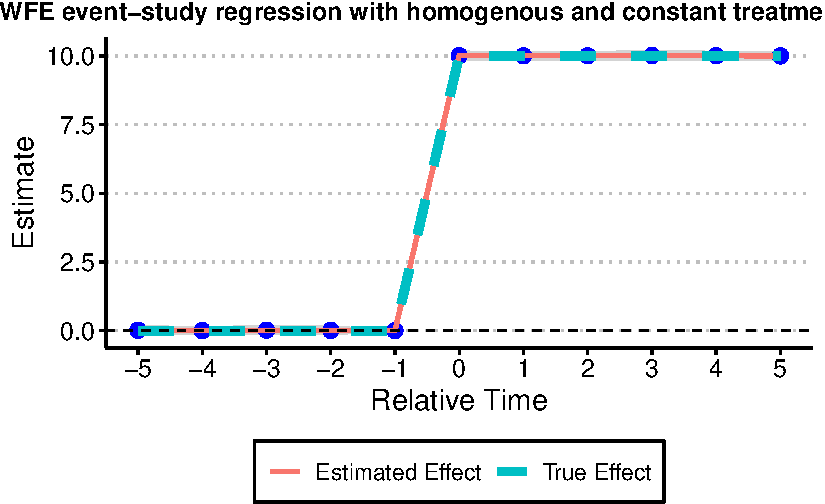
\includegraphics[keepaspectratio]{report_files/figure-pdf/unnamed-chunk-11-1.pdf}}




\end{document}
